\chapter{Quantitative Measurement of Intrinsic GTP Hydrolysis for
Carcinogenic Glutamine 61 Mutants in H-Ras} \label{ras}

\newcommand{\RalBSCN}{{Ral\textbeta{}I18C$_{\text{SCN}}$}}
\newcommand{\RalB}{{Ral\textbeta{}}}


%Mutations of human oncoprotein p$^{21}$H-Ras (hereafter ``Ras'') at glutamine 61 are known to slow the rate of guanosine triphosphate (GTP) hydrolysis and transform healthy cells into malignant cells. 
%It has been hypothesized that this glutamine plays a role in the intrinsic mechanism of GTP hydrolysis by interacting with an active site water molecule that stabilizes the formation of the charged transition state at the $\gamma$-phosphate during hydrolysis.
%However, there is no comprehensive data set of the effects of mutations to Q61 on the protein's intrinsic catalytic rate, structure, or interactions with water at the active site. 
%Here, we present the first comprehensive and quantitative set of initial rates of intrinsic hydrolysis for all stable variants of RasQ61X. 
%We further conducted enhanced molecular dynamics (MD) simulations of each construct to determine the solvent accessible surface area (SASA) of the side chain at position 61 and compared these results to previously measured changes in electric fields caused by RasQ61X mutations. 
%For polar and negatively charged residues, we found that the rates are normally distributed about an optimal electrostatic contribution, close to that of the native Q61 residue, and the rates are strongly correlated to the number of waters in the active site. 
%Together, these results support a mechanism of GTP hydrolysis in which Q61 stabilizes a transient hydronium ion, which then stabilizes the transition state while the $\gamma$-phosphate is undergoing nucleophilic attack by a second, catalytically active water molecule. 
%We discuss the implications of such a mechanism on future strategies for combating Ras-based cancers.

%%%%%%%%%%%%%%%%%%%%%%%%%%%%%%%%%%%%%%%%%%%%%%%%%%%%%%%%%%%%%%%%
%%%%%%%%%%%%%%%%%%%%%%%%%%%%%%%%%%%%%%%%%%%%%%%%%%%%%%%%%%%%%%%%
\section{Publication note} \label{ras-pub-note}
%%%%%%%%%%%%%%%%%%%%%%%%%%%%%%%%%%%%%%%%%%%%%%%%%%%%%%%%%%%%%%%%
%%%%%%%%%%%%%%%%%%%%%%%%%%%%%%%%%%%%%%%%%%%%%%%%%%%%%%%%%%%%%%%%

Portions of this chapter are adapted from the following publication: 

\noindent Elisa T. Novelli, Jeremy T. First, Lauren J. Webb; Quantitative Measurement of Intrinsic GTP Hydrolysis for Carcinogenic Glutamine 61 Mutants in H-Ras. \emph{Biochemistry}. \textbf{2018}, \emph{57}, 6356-6366.

JTF performed all calculations.
All code, force field parameters, structures, and other starting files used for the simulation, analysis, processing of data, and figure generation can be accessed at:
\url{https://github.com/jeremyfirst22/RasRal}. 
ETN performed all experiments. The experimental methods are ommited from this Chapter, but they may be found in the publication.

%%%%%%%%%%%%%%%%%%%%%%%%%%%%%%%%%%%%%%%%%%%%%%%%%%%%%%%%%%%%%%%%
%%%%%%%%%%%%%%%%%%%%%%%%%%%%%%%%%%%%%%%%%%%%%%%%%%%%%%%%%%%%%%%%
\section{Introduction} \label{ras-intro}
%%%%%%%%%%%%%%%%%%%%%%%%%%%%%%%%%%%%%%%%%%%%%%%%%%%%%%%%%%%%%%%%
%%%%%%%%%%%%%%%%%%%%%%%%%%%%%%%%%%%%%%%%%%%%%%%%%%%%%%%%%%%%%%%%

The Ras superfamily of approximately 150 GTPases consists of signaling proteins that hydrolyze guanosine triphosphate (GTP) to guanosine diphosphate (GDP) to switch between ON (GTP-bound) and OFF (GDP-bound) states in a variety of signal transduction pathways \cite{Bourne1991, Krauss2003}.
There are multiple inputs and outputs in this catalytic cycle: (1) Ras-like GTPases interact with multiple downstream effector proteins to facilitate signaling in the ON state and propagate a signaling cascade; (2) GTPase activating proteins (GAPs) bind to Ras and facilitate GTP hydrolysis, converting Ras to the OFF state; and (3) exchange factor proteins (GEFs) bind to Ras to promote the exchange of GDP for GTP to return Ras to the ON state \cite{Krauss2003, Cherfils2013, Khrenova2015}.
A canonical member of this superfamily, p$^{21}$H-Ras (hereafter ``Ras''), is part of a signaling pathway that regulates cell survival and proliferation \cite{Shields2000, Cox2003, Downward2003, Repasky2004, Prior2012}.
Mutations to Ras that slow hydrolysis and leave the protein in an ON state can lead to uncontrolled cell growth and tumorigenesis \cite{Prior2012}. 
A recent survey found that mutations to the Ras family of genes appear in approximately 16\% of cancer tumors, with some specific types such as pancreatic tumors showing far greater mutation frequencies \cite{Prior2012}. 
Because of its role as a molecular switch, the oncogenic properties of Ras are intimately tied to the kinetics of the GTP hydrolysis reaction.

Since the discovery of Ras in 1964\cite{Harvey1964}, three key residues have been identified that, when mutated, are present in the vast majority of Ras-induced tumor cells: G12, G13, and Q61 \cite{Prior2012}.
The effects of mutations to the native glycine residues at positions 12 and 13 have been well studied and are largely considered to result from steric effects on the folding and dynamics of the enzyme near the active site \cite{Prior2012, Bos1989, Eccleston1993, Hobbs2016}.
However, the role of Q61 in the hydrolysis mechanism is more puzzling and has been debated continuously in the literature \cite{Kamerlin2013, Carvalho2015}.
In a crystal structure solved in 1990, Pai et al. observed a water molecule that was positioned for in-line nucleophilic attack on the leaving phosphate group and postulated that Q61 acts as a general base to deprotonate the attacking water molecule and activate it for GTP hydrolysis \cite{Pai1990}. 
However, using theoretical calculations, Langen et al. demonstrated in 1992 that Q61 cannot act as the general base in such a mechanism because the activation energy for proton abstraction is too large to be consistent with the observed rate \cite{Langen1992}.
Further, in 2004, Shurki and Warshel\cite{Shurki2004} demonstrated that Q61 plays an indirect but significant role in the RasGAP-mediated mechanism of GTP hydrolysis by ``pre-organizing'' the active site of Ras to allow Arg789 of RasGAP (referred to as the ``arginine finger'') to insert into the active site and stabilize the transition state of the nucleophilic attack by water \cite{Scheffzek1997}. 
This RasGAP activity increases the hydrolysis reaction rate by a factor of $10^5$ \cite{Schweins1995}.
This mechanism of assisted hydrolysis has since been further studied and characterized \cite{Khrenova2015, Shurki2004, Grigorenko2005}.

However, the affinity of RasGAP for Ras is 3 orders of magnitude lower than that of Ras and its downstream effectors\cite{Vogel1988}, and so \emph{in vivo} Ras is primarily docked with a downstream effector. 
Because of this, therapeutic strategies for RasQ61X mutations must consider the protein when it is bound to its downstream effector, and thus GTP hydrolysis mostly occurs through an intrinsic, not assisted, mechanism. 
However, the molecular level details of this intrinsic mechanism of hydrolysis have remained elusive.

In 2010, Buhrman et al. proposed a new mechanism for intrinsic hydrolysis involving two water molecules, in which the catalytic water shuttles a proton to a bridging water molecule that is stabilized by hydrogen bonds to Q61 and Y32\cite{Buhrman2010}, as illustrated in Figure \ref{fig:ras-mech}A. 
This positively charged hydronium ion stabilizes the transition state in the intrinsic mechanism and partially fulfills the role of the ``arginine finger'' in the RasGAP-assisted hydrolysis mechanism, although with much lower efficacy. 
From this perspective, the role of Q61 is to stabilize the hydronium ion, which in turn stabilizes the transition state. 
This mechanism was suggested based on the appearance of a crystallographic water molecule in the pdb structure 3k8y\cite{Buhrman2010} but has not been confirmed through other experiments. 
However, it is further supported by the fact that, in separate work, the same group found that highly and moderately transforming (cancer causing) mutants of Q61 tended to be buried and occluded from solvent, while weakly and nontransforming (noncancer causing) mutations were solvent exposed \cite{Buhrman2007}. 
This supports the idea that water is crucial to the intrinsic hydrolysis mechanism. If this hypothesis is correct, then Q61 can be thought of as participating electrostatically, not chemically, in GTP hydrolysis, and so a careful interrogation of the effects of the electric field in and around the active site at steady-state and during hydrolysis are important for proving this mechanism.

\begin{figure}
    \center
    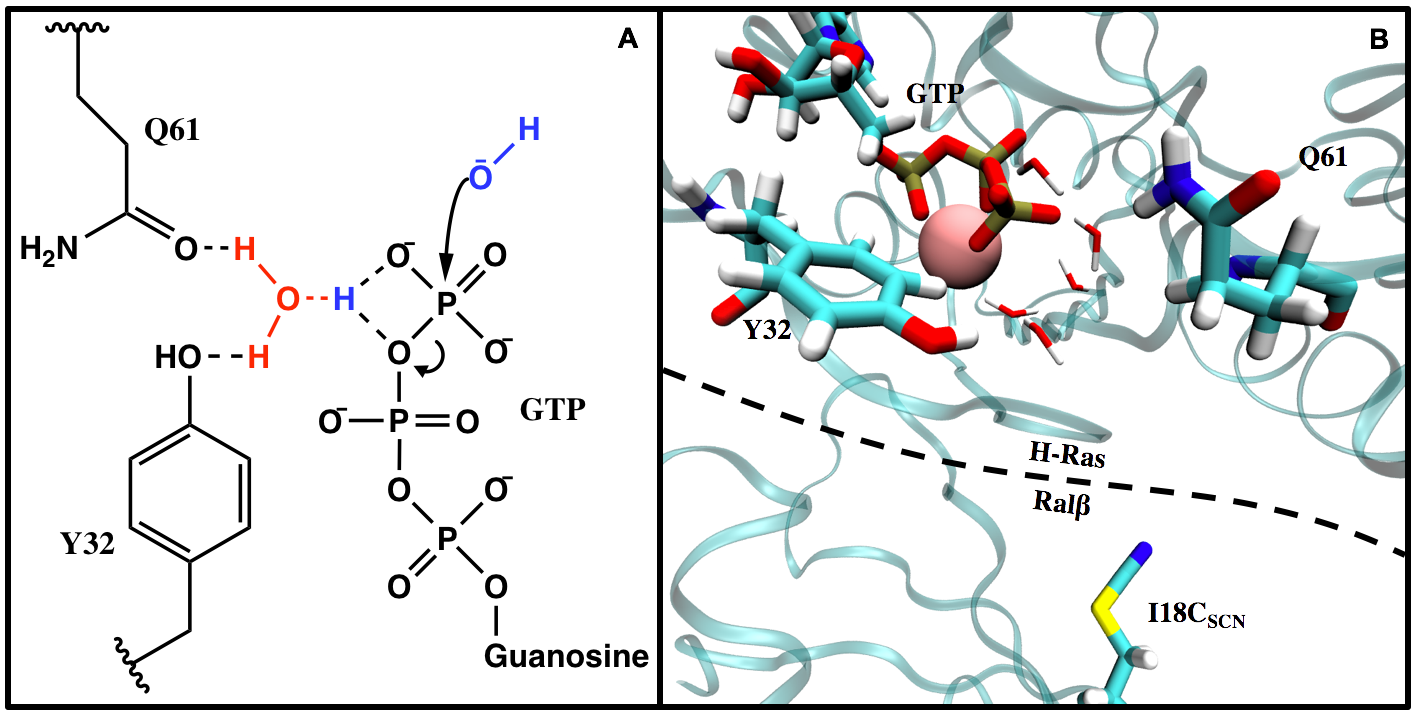
\includegraphics[width=\double]{figures-ras/Figure1_two_column.png}
    \caption[Proposed Ras hydrolysis mechanism and illustration of system]{
        (A) A proposed multiwater mechanism of the intrinsic Ras GTPase reaction. 
        The catalytic water (blue) shuttles a proton to a nearby, stabilized water (red) via the $\gamma$-phosphate, adopted from ref \citenum{Buhrman2010} and ref \citenum{Stafford2012}. 
        (B) A snapshot of the Ras/\RalBSCN{} interface. 
        The ribbons in the background represent the backbone of the protein. 
        The sticks represent the relevant residues in the system: Y32 of Ras, Q61 of Ras, GTP, and \RalBSCN{}. 
        The pink sphere is \ce{Mg^2+}, and the small sticks represent water in the active site.
    }
    \label{fig:ras-mech}
\end{figure}

Previous work in our group has made use of vibrational Stark effect (VSE) spectroscopy to interrogate the electric field of the active site of Ras constructs with mutations at position 61 (RasQ61X, where X represents a mutation from the native Gln residue) \cite{Stafford2012}.
VSE spectroscopy takes advantage of the difference dipole moment, $\Delta\vec{\mu}$, inherent in small vibrational probes (in this case a nitrile), to relate shifts in the vibrational frequency, $\Delta E$, to changes in local electric field, $\Delta\vec{F}$, according to eq \ref{eq:ras-stark} \cite{Andrews2000, Andrews2002, Fafarman2006, Fried2015, Slocum2018}:

\begin{equation}
\Delta E = - \Delta\vec{\mu}\cdot\Delta\vec{F}
\label{eq:ras-stark}
\end{equation}

In that work, a nitrile probe was strategically incorporated at position 18 of the Ras binding domain of the downstream effector RalGDS (hereafter, \RalB{}), generating the construct \RalBSCN{} which denotes that the native isoleucine at position 18 was replaced with a cysteine, which was then post-translationally modified to cyanocysteine. 
Though a different protein, c-Raf kinase (Raf), is the primary downstream effector of Ras \emph{in vivo}, Raf has been shown to alter some rates of intrinsic hydrolysis \cite{Buhrman2011}.
By docking \RalBSCN{} with Ras, the nitrile group was well positioned to report on electric field changes due to mutations to Q61 in and around the Ras active site, without affecting the intrinsic hydrolysis mechanism. 
A snapshot of this system based on the pdb structure 1lfd is shown in Figure \ref{fig:ras-mech}B.

While nitrile spectra have also been shown to report on solvation environments due to quantum mechanical effects of specific hydrogen bonding \cite{Waegele2009, Oh2008,Fafarman2010}, here we show that the solvent exposure and specific hydrogen bonding interactions of the nitrile on \RalBSCN{} are identical between the Ras mutants. 
We therefore interpreted the shifts in vibrational frequency of the nitrile probe on \RalB{} as changes in local electric field, according to eq \ref{eq:ras-stark}, caused by mutations to Q61 in Ras across the protein-protein interface ($\sim$9 \si{\angstrom}). 
Because any multiwater intrinsic hydrolysis mechanism, such as that proposed by Buhrman et al., relies on noncovalent stabilization of water in the active site, we compared the shifts in nitrile frequency to quantitative measurements of the ability of the side chain to interact with water. 
We observed correlations between the nitrile shifts and both the solvent accessible surface area (SASA) and the hydration potential of the residue at position 61 \cite{Stafford2012}.
Based on these results, we hypothesized that the identity of the residue at position 61 affects the rate of intrinsic GTP hydrolysis through noncovalent and electrostatic stabilization of water molecules according to each residue's affinity for water, supporting a multiwater mechanism such as the one proposed in Figure \ref{fig:ras-mech}A.

In spite of the ongoing debate regarding the role of Q61 in the mechanism of intrinsic hydrolysis, there has not yet been a comprehensive quantitative examination of the role of Q61 mutations on the intrinsic hydrolysis rate. 
Though the literature has suggested that at least 17 Q61X intrinsic hydrolysis rates have been measured, most have not been explicitly reported and, to our knowledge, were measured only semiquantitatively \cite{Der1986}.
Fully quantitative intrinsic hydrolysis rate constants of RasQ61X mutations have only been reported for WT, E, H, and L \cite{Krengel1990, Frech1994}.

Here, we present measurements of the initial rate of intrinsic hydrolysis of GTP in WT and 17 RasQ61X constructs. 
Intrinsic rates were measured using a malachite green colorimetric assay based on the binding of malachite green indicator to a phosphomolybdate complex formed from the phosphate product of the hydrolysis reaction. 
This GTPase activity assay is useful because it is a sensitive and nonradioactive technique for detecting phosphate and has been successfully applied to other GTPase proteins \cite{Quan2005}.
To our knowledge, this is the first report of a comprehensive set of quantitative kinetics data for all Q61X mutations (except Q61P and Q61C, which could not be expressed). 
Our initial rate measurements indicated that, in most cases, mutations to position 61 resulted in significantly slower GTP hydrolysis. 
We compared our measured initial rates to previously published information on the electric field due to these mutations, measured by VSE spectroscopy \cite{Stafford2012}.
We found that the initial rate of intrinsic hydrolysis was related to the observed nitrile frequencies for residues that are able to stabilize the hypothesized hydronium ion (polar and negatively charged residues). 
No relationships were observed for amino acids with positively charged or nonpolar side chains.

Additionally, we used enhanced molecular dynamics (MD) simulations to determine the molecular basis for this relationship by calculating the SASA of the polar side chain atoms as well as the entire side chain of Q61X. 
We found that the reported vibrational frequencies were well correlated to the SASA of the side chain polar atoms in all polar and charged amino acids, while the initial rate of intrinsic hydrolysis was well correlated to the SASA of the entire side chain, but only for polar and negatively charged amino acids. 
For the polar and negatively charged residues, we found a strong correlation between the number of water molecules in the active site (determined from MD) and the initial rate of intrinsic hydrolysis.
This evidence strongly supports a multiwater mechanism, such as the mechanism proposed by Buhrman et al. and illustrated in Figure \ref{fig:ras-mech}A, where a positively charged hydronium ion stabilizes the transition state of the reaction. 
This kinetic data set is invaluable for understanding the intrinsic mechanism of hydrolysis and will provide insight for further computation and development of therapeutic strategies


%%%%%%%%%%%%%%%%%%%%%%%%%%%%%%%%%%%%%%%%%%%%%%%%%%%%%%%%%%%%%%%%
%%%%%%%%%%%%%%%%%%%%%%%%%%%%%%%%%%%%%%%%%%%%%%%%%%%%%%%%%%%%%%%%
\section{Materials and methods} \label{ras-methods}
%%%%%%%%%%%%%%%%%%%%%%%%%%%%%%%%%%%%%%%%%%%%%%%%%%%%%%%%%%%%%%%%
%%%%%%%%%%%%%%%%%%%%%%%%%%%%%%%%%%%%%%%%%%%%%%%%%%%%%%%%%%%%%%%%

%\subsection{Mutagenesis}
%
%The gene for hexahistidine-tagged WT H-Ras, residues 1-166, was a gift of the Kuriyan laboratory \cite{Boriack-Sjodin1998}. 
%A plasmid containing hexahistidine-tagged Tobacco Etch Virus Protease (His-TEV) with the S219V mutation in \emph{E. coli} Bl21(DE3)-RIL cells was a gift from David Waugh (Addgene plasmid 8827) \cite{Kapust2001}. 
%The 97-residue Ras Binding Domain of \RalB{} was taken from residues 790-886 of RalGDS and numbered according to the pdb entry 1lfd \cite{Huang1998}. 
%The gene was cloned and mutated as described previously \cite{Stafford2012, Stafford2010}.
%Mutations to Q61 of Ras were made using the Quikchange Lightning site-directed mutagenesis kit (Agilent).
%
%\subsection{Purification}
%
%Plasmids encoding the WT and mutant Ras constructs were transformed into BL21(DE3) cells for expression. 
%All proteins were expressed and purified as previously described \cite{Stafford2012, Kapust2001, Stafford2010}, with the exception of the buffers used for Ras, which were altered to minimize phosphate background in the kinetics experiments. 
%All reagents were purchased from Sigma-Aldrich and used without further purification unless stated otherwise. 
%Briefly, cells were collected and resuspended in loading buffer (50 mM Tris-HCl, 250 mM NaCl, 40 mM imidazole, 10\% glycerol, pH 7.5) for lysis via probe sonication followed by centrifugation to remove cell debris. 
%The supernatant was loaded onto a nickel immobilized metal affinity column (Ni-IMAC, Fisher). 
%His-tagged Ras proteins were eluted with an elution buffer (50 mM Tris-HCl, 250 mM NaCl, 500 mM imidazole, 10\% glycerol, pH 7.5). 
%Protein was exchanged into a cleavage buffer (50 mM Tris, 50 mM KCl, 10\% glycerol, pH 8) with a PD-10 column (GE Healthcare) and cleaved with His-TEV at a ratio of approximately 1 mg His-TEV to 100 mg of His-Ras overnight at 4 \si{\celsius}. His-TEV and uncleaved Ras were removed by passing the solution through another Ni-IMAC column, and the cleaved protein was exchanged into final buffer (50 mM Tris, 100 mM NaCl, 10\% glycerol, pH 7.5) and either used immediately or flash frozen and stored at -80 \si{\celsius} for later use. 
%To ensure that the active site of Ras contained GDP (OFF state) in preparation for kinetics experiments, the purified Ras was incubated with 5 mM dithiothreitol (DTT), 5 mM ethylenediamine tetraacetic acid (EDTA), and GDP in 100-fold excess of the protein concentration for 90 min on ice, and then 10 mM \ce{MgCl2} was added and the solution incubated for a further 30 min on ice. 
%The GDP-containing protein was then buffer exchanged into kinetics buffer (50 mM Tris-HCl, 50 mM NaCl, 20 mM EDTA, 5 mM \ce{MgCl2}, 0.01\% Triton X-100, pH 7.5) for the kinetics experiments. 
%The RasQ61C and RasQ61P mutations could not be expressed for reasons we have not investigated and are thus not presented here. 
%The nitrile functional group on \RalB{} was introduced as previously described \cite{Stafford2010}.
%
%\subsection{Kinetics}
%
%The initial rates of hydrolysis of GTP by RasQ61X constructs were measured using the malachite green assay\cite{Quan2005, Hohenwallner1973, Lanzetta1979} to detect the production of inorganic phosphate. 
%The hydrolysis product, \ce{Pi}, was detected through the formation of a colorless phosphomolybdate complex under acidic conditions, which reacted with malachite green indicator to form a colored product that was quantified by UV-vis absorption at 640 nm. 
%The assay has a broad dynamic range (typically 1-200 $\mu$M) that was tailored to the reaction conditions based on the ratio of assay volume to malachite green detection reagent volume. 
%The assay has the advantage of using GTP as the substrate instead of fluorescently labeled GTP, which introduces kinetic artifacts, or radiolabeled GTP, which has associated handling hazards and expenses.
%
%The malachite green reagent contained ammonium molybdate and malachite green oxalate dissolved in 1 N HCl (all purchased from Sigma-Aldrich) and was made as described previously \cite{Quan2005}.
%A 1 mM phosphate standard stock solution was made by drying the highest available purity \ce{K3PO4} in an oven at 110 \si{\celsius} overnight before dissolving in high purity water. 
%Lower concentration standard solutions of \ce{K3PO4} for the calibration curve were serially diluted from the stock solution in kinetics buffer at the time of the experiment. 
%The GTP substrate solution contained 40 $\mu$M GTP and 1 mM DTT in kinetics buffer. 
%To minimize contamination that increased the phosphate background, we used the highest purity GTP available. 
%Each reaction was initiated by mixing 20 $\mu$L of 8 mM RasQ61X with 20 $\mu$L of GTP substrate solution for a final assay reaction solution of 4 $\mu$M RasQ61X and 20 $\mu$M GTP. 
%Reactions were incubated at 37 \si{\celsius} from 0 to 8 h by initiating the 8 h reaction first and then adding subsequent reactions to the incubator at each time point. 
%All reactions were then transferred to a black, optical-bottom 384-well plate (Thermo Scientific) and all stopped at the same time through the addition of the malachite green reagent. 
%Reactions were done at least in triplicate, and each reaction vial had enough volume for three wells, resulting in at least 9 measurements for each time point. 
%Each well contained 10 $\mu$L of assay reaction and 30 $\mu$L of malachite reagent, and the optical response was linear (Figure \ref{fig:ras-response}) through the entire range of standards (0-25 $\mu$M phosphate). 
%Absorption of the phosphomolybdate/malachite green colored complex was measured via a BioTek Synergy H4 plate reader at 640 nm using path length correction functionality to account for small differences in volume due to pipetting error.
%
%\begin{figure}
%    \center
%    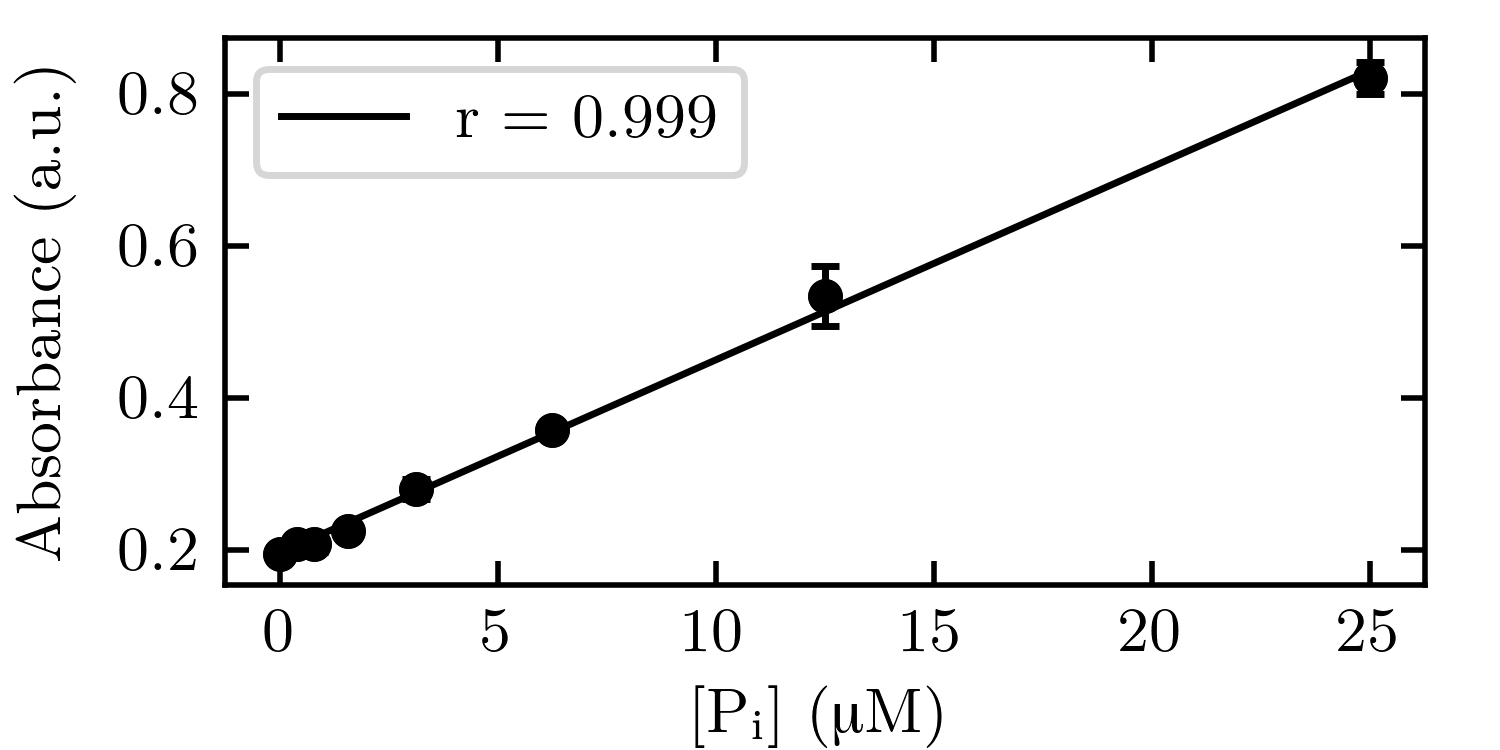
\includegraphics[width=\single]{figures-ras/optical_response.png}
%    \caption[Calibration curve of the malachite green colorimetric assay]{
%        Calibration curve of the malachite green colorimetric assay collected from phosphate standards of 0.00, 0.39, 0.78, 1.56, 3.13, 6.25, 12.5, and 25 $\mu$M. 
%        The response is linear over the range of phosphate concentration measured in our experiments.
%    }
%    \label{fig:ras-response}
%
%\end{figure}

\subsection{MD and SASA calculations} 

A template Ras/\RalB{}I18C docked complex with GTP and \ce{Mg^2+} in the binding site and all crystallized waters was modeled by homology from the 1lfd crystal structure\cite{Huang1998} using the MODELLER software package \cite{Marti-Renom2000, Sali1993, Fiser2000}, and the E31K mutation on Ras in the published structure was reverted to the wild-type glutamate. 
From this structure, I18C of \RalB{} was further modified to cyanocysteine and independently minimized using the Avogadro molecular editing package \cite{Hanwell2012}. 
Using this template, 15 separate mutations from the WT Q61 residue of Ras to all residues except A, G, C, and P were made using the mutagenesis wizard tool in PyMol \cite{DeLano2002}.
Mutations to A and G were not made because they lack a $\chi_1$ dihedral angle. 
Mutations to C and P were not made because the rates could not be measured experimentally.
Parameters for the nitrile-containing cyanocysteine (CNC) residue have been described previously \cite{Stafford2010, Ensign2011}.
Phosphate parameters for use in GTP have been published by Meagher et al\cite{Meagher2003}.
However, the charges in this parameter set were derived in accordance with the Amber99 force field. 
To attain parameters consistent with the Amber03 force field (ffAmber03), multiconformational RESP\cite{Cornell1993, Bayly1993, Cieplak1995} was used to fit charges using the Duan et al. protocol\cite{Duan2003} in the seven minimum energy conformations identified in Meagher et al. 
Charges for ffAmber03 were all similar to the charges for the Amber99 force field and can be found in Table \ref{tbl:ras-charges}. 
Though the protonation state of the terminal phosphate of GTP in Ras proteins has been recently discussed in the literature \cite{Knihtila2015, Mann2018}, for these simulations we used the fully deprotonated structure of GTP (net charge of -4). 
All further minimizations and MD simulations were performed using the Gromacs 2016.3 molecular dynamics simulation package\cite{Berendsen1995, Lindahl2001, VanDerSpoel2005, Miyake-Stoner2009, Hess2008, Pronk2013, Pall2015, Abraham2015} and ffAmber03 \cite{Duan2003, Sorin2005}.

\begin{table}
    \caption[Partial charges for phosphate atoms]{
        Partial charges for the phosphate atoms derived in accordance with Amber03.
    }
    \begin{center}
    \begin{tabular}{cc}
    \toprule
       \rowcolor{lgray}
       Atom Name & Charge  \\
        \cmidrule(r){1-1}\cmidrule(l){2-2}
     CT  &        0.295166 \\
      HC &        -0.034122 \\
     O3  &       -0.934008   \\
     O2(1)  &   -0.841563   \\
     O2(2) &    -0.854716   \\
     OS(1)  &   -0.471014   \\
     OS(2)  &   -0.506642   \\
     OS(3) &    -0.529221   \\
     P(1)   &     1.190429   \\
     P(2)   &     1.178895   \\
     P(3)   &     1.139338   \\
    \bottomrule
    \end{tabular}
    \end{center}
    \label{tbl:ras-charges}
\end{table}

The 16 protein systems were energy minimized in a vacuum using the steepest descent algorithm and solvated in a dodecahedron box of TIP3P water \cite{Jorgensen1983}, with a minimum distance of 1.5 nm between the protein and the edge of the box. 
The solvated systems were then energy minimized using steepest descent, heated under the NVT ensemble at 300 K, and equilibrated under the NPT ensemble at 1 atm, each with heavy atom restraints on the protein atoms. 
Following equilibration, the heavy atom restraints were removed, and a dihedral restraint of 100 kJ mol$^{-1}$ was applied to the $\chi_1$ dihedral of Q61X in 12 windows separated by \ang{30}. 
Each of these restrained windows was relaxed in the NVT ensemble for 50 ps to allow the dihedral angle to move to the sampling window, resulting in 12 equilibrated rotamers of Q61 per each mutation at this residue (192 total structures). 
The dihedral restraint on the $chi_1$ dihedral of Q61X was relaxed to 70 kJ mol$^{-1}$ and given a flat potential within \ang{15} of the window of interest, and production MD was run on each equilibrated structure for 2 ns, using a 2 fs time step and a stochastic integrator. 
Particle mesh-Ewald electrostatics\cite{Cheatham1995} was implemented with a Coulombic cutoff of 8 \si{\angstrom}, and van der Waals (VDW) interactions were cut off at 8 \si{\angstrom}. 
Snapshots were recorded every 4 ps during simulations.

%%%%%%%%%%%%%%%%%%%%%%%%%%%%%%%%%%%%%%%%%%%%%%%%%%%%%%%%%%%%%%%%
%%%%%%%%%%%%%%%%%%%%%%%%%%%%%%%%%%%%%%%%%%%%%%%%%%%%%%%%%%%%%%%%
\section{Results} \label{ras-results}
%%%%%%%%%%%%%%%%%%%%%%%%%%%%%%%%%%%%%%%%%%%%%%%%%%%%%%%%%%%%%%%%
%%%%%%%%%%%%%%%%%%%%%%%%%%%%%%%%%%%%%%%%%%%%%%%%%%%%%%%%%%%%%%%%

\subsection{Measurement of the intrinsic hydrolysis rate}

A hypothesized mechanism for intrinsic GTP hydrolysis by Ras (Figure \ref{fig:ras-mech}A) proposes that the electric field created by the arrangement of amino acids at the Ras surface is critically important for enzyme function. 
To determine the effect that each Q61X mutation caused to the local electric field, it was necessary to determine the extent to which each mutation changed the rate of enzyme hydrolysis, which was not possible to construct from the literature. 
Various methods used previously on different RasQ61X mutants have not been comprehensive or quantitative, but generally it has been found that mutations to position 61 result in slower intrinsic GTP hydrolysis rates \cite{Der1986, Krengel1990}. 
We measured the initial rate of intrinsic hydrolysis of WT Ras and 17 mutants at position 61 to examine the role of the residue in the electrostatic stabilization of the proposed hydronium ion. 
To do this, we monitored the increase in concentration of phosphate over time for each mutant, measured using a malachite green colorimetric assay. 
Because the Ras-GTP complex has a $K_d$ in the picomolar range, the addition of excess GTP to initiate the reaction resulted in a single exponential rise in the concentration of phosphate. 
In order to have a quantitative comparison between the mutants in our experiment, we used linear regression on the first five measurements of phosphate concentration (i.e., 0-180 min), which corresponds to the linear portion of the exponential curve. 
We extracted the initial rates from the slope of the resulting fits, and all fits are shown in Figure \ref{fig:ras-all_fits}. 
For brevity, representative curves are shown in Figure \ref{fig:ras-curves}, and initial rates for all mutants are reported in Table \ref{tbl:ras-data}. 
The error is reported as the standard error of the linear regression. 
In some cases, we obtained a better fit with smaller error by omitting the first data point because of low sensitivity of the zero time point in colorimetric assays. 
In all cases, we report the fit that yielded the lowest standard error. 
We chose to measure the initial rate of the reaction rather than a fit of the observed rate over the entire exponential curve because some mutants do not appear to have reached equilibrium through the course of the 8 h experiment, either because the mutant is too slow or because the mutant protein no longer functions due to denaturation or aggregation. 
However, it should be noted that only the Q61V construct visibly precipitated after 3 h at 37 \si{\celsius}, and there was no other visible aggregation for any other mutant over the course of the 8 h experiment.

\begin{figure} 
    \center
    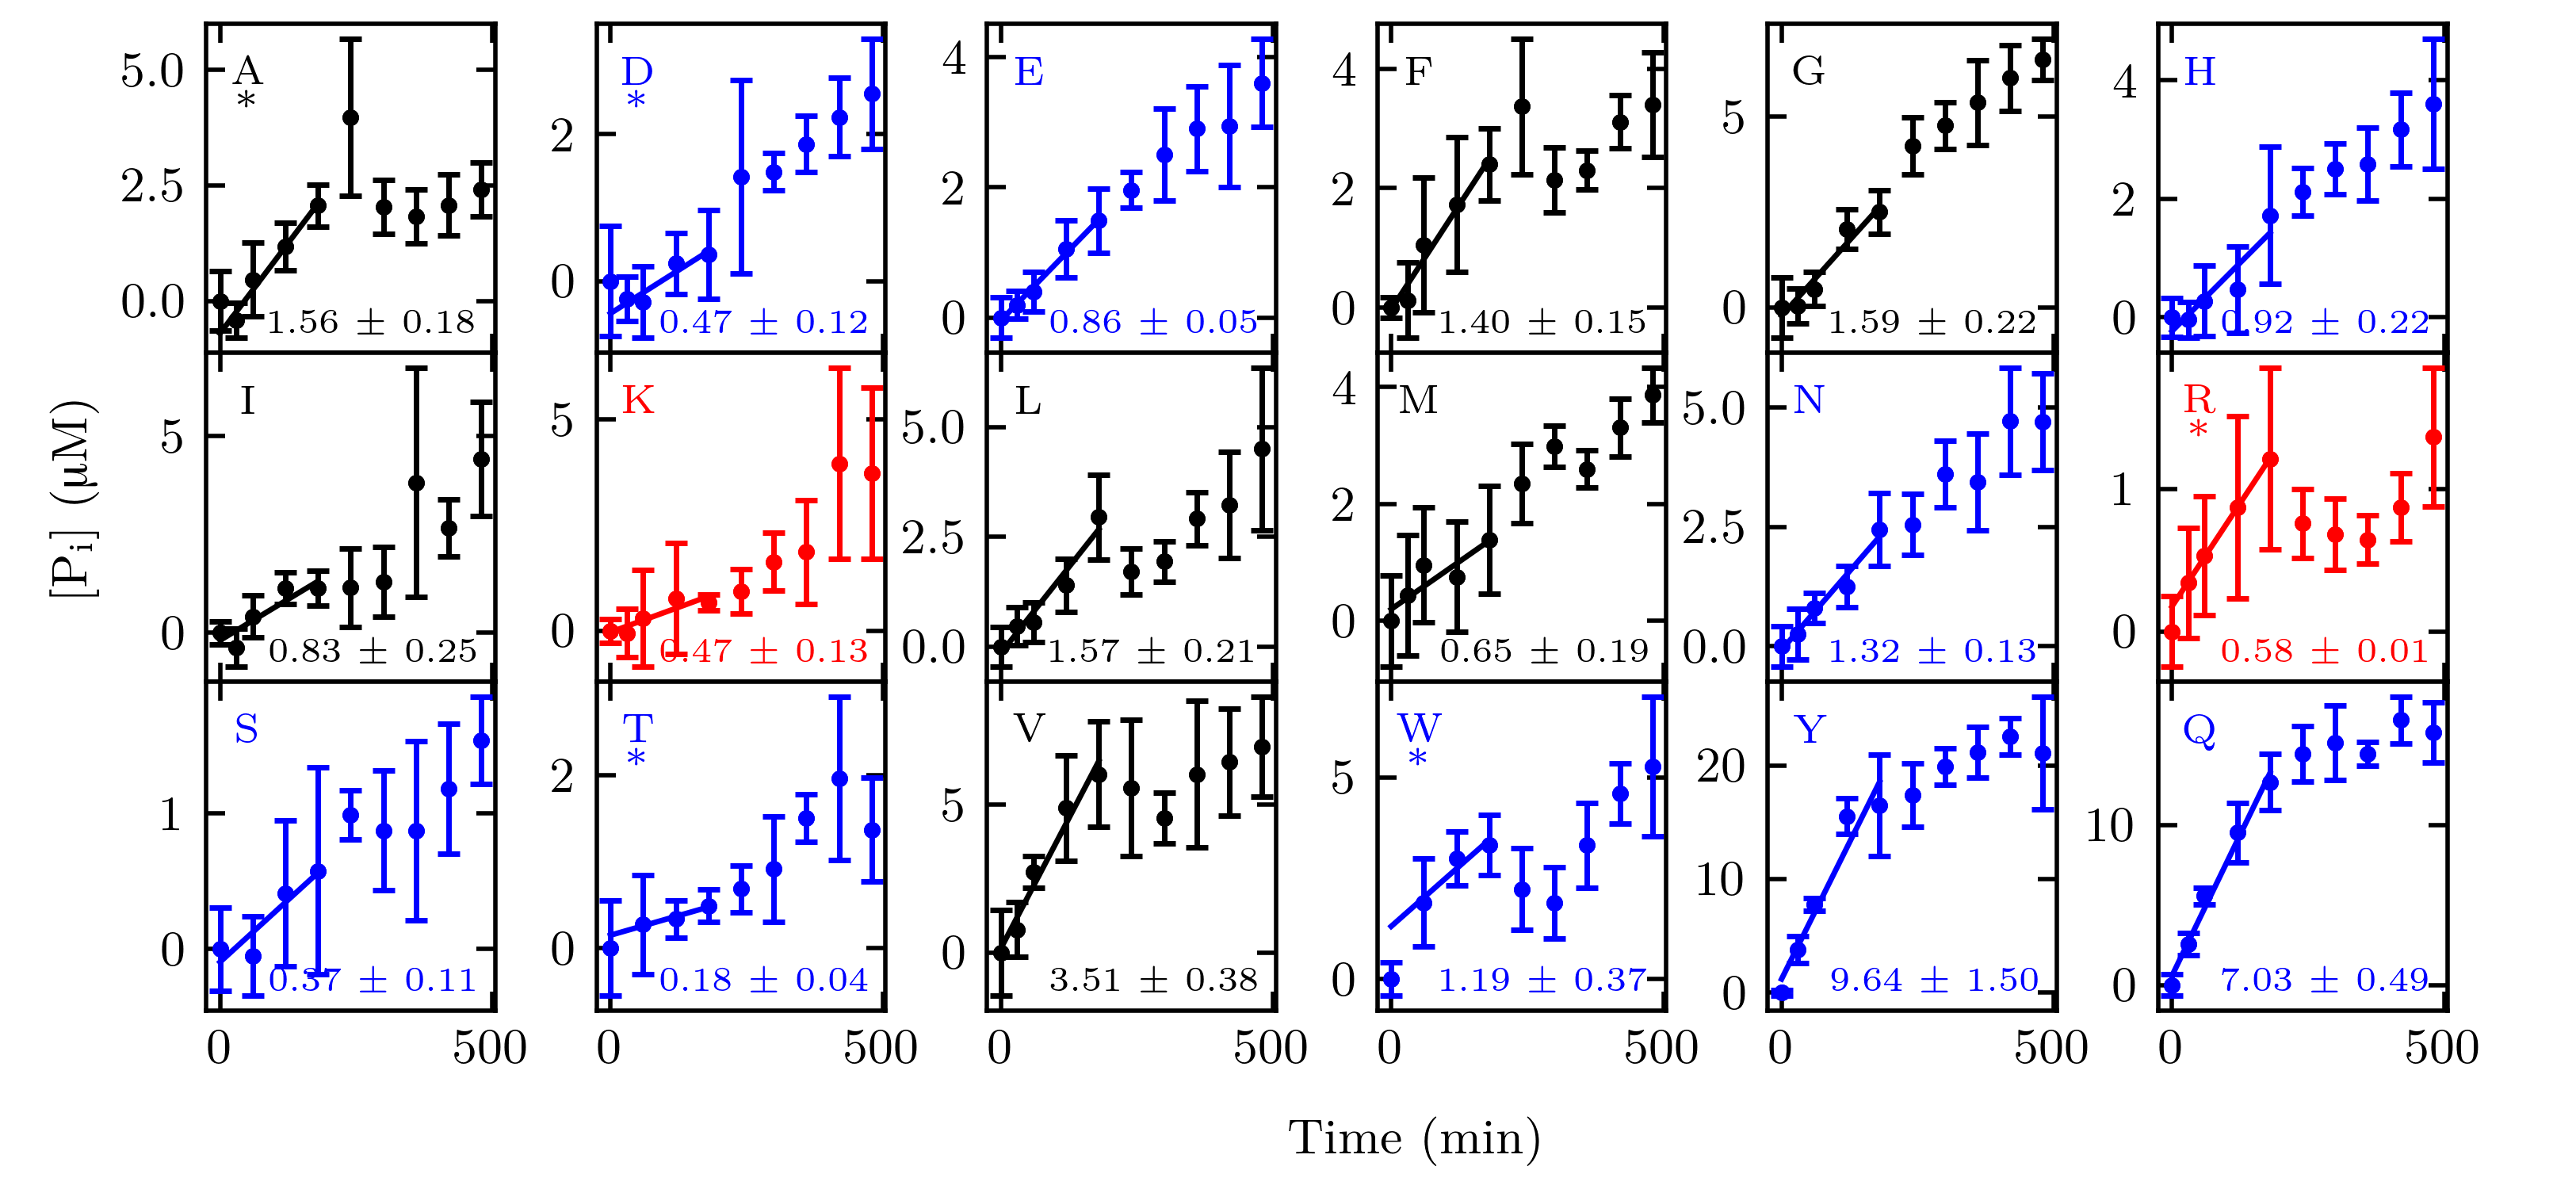
\includegraphics[width=\double]{figures-ras/all_fits.png}
    \caption[Phosphate production in each RasQ61X mutant]{
        The production of inorganic phosphate, P$_\text{i}$, as a function of reaction time for all viable RasQ61X constructs. 
        The identity of the amino acid at position 61 is shown in the upper left corner of each plot. 
        The first five points were fit with linear regression. 
        The slope and standard error of the fit are displayed in the bottom-right corner of each window. 
        If a lower standard error was obtained by omitting the first time point (0 min), then that fit is reported. 
        Such cases are marked with an asterisk in the top-left corner. 
        Blue: polar or negatively charged residues; red: positively charged residues; black: nonpolar residues.
    }
    \label{fig:ras-all_fits}
\end{figure}

\begin{table}
    \caption[Summary of experimental and computational results]{
        Vibrational Frequencies of a Nearby Nitrile on \RalBSCN{}, 
        Measured Intrinsic Initial Rates of GTP hydrolysis, and 
        Computed SASA Values of Both the Entire Side Chain and Only the Side Chain Polar Atoms (N, O, and H bound to N or O) from MD Simulation for 18 Constructs of RasQ61X
    }
    \begin{center}
    \begin{tabular}{ccccc}
    \toprule
    \rowcolor{lgray}
        Ras Construct & $\tilde{\nu}^{a}$   & Initial Rate$^{b}$  & \multicolumn{2}{c}{SASA$^{c}$ of: (\si{\angstrom^2}) }\\
    \rowcolor{lgray}
    & (cm$^{-1}$) &     ($10^{-2}$ $\mu$M min$^{-1}$)  & polar atoms & side chain \\
    \cmidrule(r){1-1}\cmidrule(lr){2-2}\cmidrule(lr){3-3}\cmidrule(l){4-5}
    WT Ras$^{d}$   & $2162.8 \pm 0.2$ & $ 7.03 \pm 0.49  $ & $65 \pm 15$ & $98  \pm 16 $\\
    \rowcolor{lgray}
    \multicolumn{5}{c}{Residues with Charged Sidechains} \\
    RasQ61D & $2162.0 \pm 0.1$ & $ 0.47 \pm  0.12 $ & $51 \pm 7  $ & $77  \pm 7  $\\
    RasQ61E & $2162.8 \pm 0.2$ & $ 0.86 \pm  0.05 $ & $60 \pm 10.$ & $91  \pm 11 $\\
    RasQ61K & $2163.1 \pm 0.2$ & $ 0.47 \pm  0.13 $ & $50 \pm 17 $ & $114 \pm 22 $\\
    RasQ61R & $2162.4 \pm 0.1$ & $ 0.58 \pm  0.01 $ & $71 \pm 24 $ & $121 \pm 24 $\\
    \rowcolor{lgray}
    \multicolumn{5}{c}{Residues with Polar Sidechains} \\
    RasQ61H & $2163.8 \pm 0.2$ & $ 0.92 \pm  0.22 $ & $34 \pm 6  $ & $108 \pm 14 $\\
    RasQ61N & $2162.7 \pm 0.2$ & $ 1.32 \pm  0.13 $ & $49 \pm 13 $ & $76  \pm 10 $\\
    RasQ61S & $2164.4 \pm 0.1$ & $ 0.37 \pm  0.11 $ & $18 \pm 9  $ & $47  \pm 9  $\\
    RasQ61T & $2164.7 \pm 0.2$ & $ 0.18 \pm  0.04 $ & $20 \pm 9  $ & $59  \pm 11 $\\
    RasQ61W & $2164.1 \pm 0.2$ & $ 1.19 \pm  0.37 $ & $18 \pm 10.$ & $151 \pm 21 $\\
    RasQ61Y & $2163.5 \pm 0.1$ & $ 9.64 \pm  1.50 $ & $36 \pm 15 $ & $130.\pm 25 $\\
    \rowcolor{lgray}
    \multicolumn{5}{c}{Residues with Nonpolar Sidechains} \\
    RasQ61A & $2162.0 \pm 0.2$ & $ 1.56 \pm  0.18 $ &                   &         \\
    RasQ61F & $2163.0 \pm 0.2$ & $ 1.40 \pm  0.15 $ & $0  \pm 0  $ & $114 \pm 21 $\\
    RasQ61G & $2163.1 \pm 0.1$ & $ 1.59 \pm  0.22 $ &              &              \\
    RasQ61I & $2164.0 \pm 0.2$ & $ 0.83 \pm  0.25 $ & $0  \pm 0  $ & $95  \pm 9  $\\      
    RasQ61L & $2163.2 \pm 0.2$ & $ 1.57 \pm  0.21 $ & $0  \pm 0  $ & $102 \pm 14 $\\
    RasQ61M & $2162.6 \pm 0.1$ & $ 0.65 \pm  0.19 $ & $0  \pm 0  $ & $101 \pm 20 $\\
    RasQ61V & $2163.9 \pm 0.0$ & $ 3.51 \pm  0.38 $ & $0  \pm 0  $ & $78  \pm 11 $\\
    \bottomrule
    \end{tabular} \\
    \end{center}
    $^{a}$Taken from ref \citenum{Stafford2012}. $^{b}$Errors in the rate are reported as the standard error of the linear fit. $^{c}$Errors in the SASA are reported as the standard deviation of the entire ensemble of structures. $^{d}$The identity of position 61 in wild-type Ras is Q.
    \label{tbl:ras-data}
\end{table}

\begin{figure}
    \center
    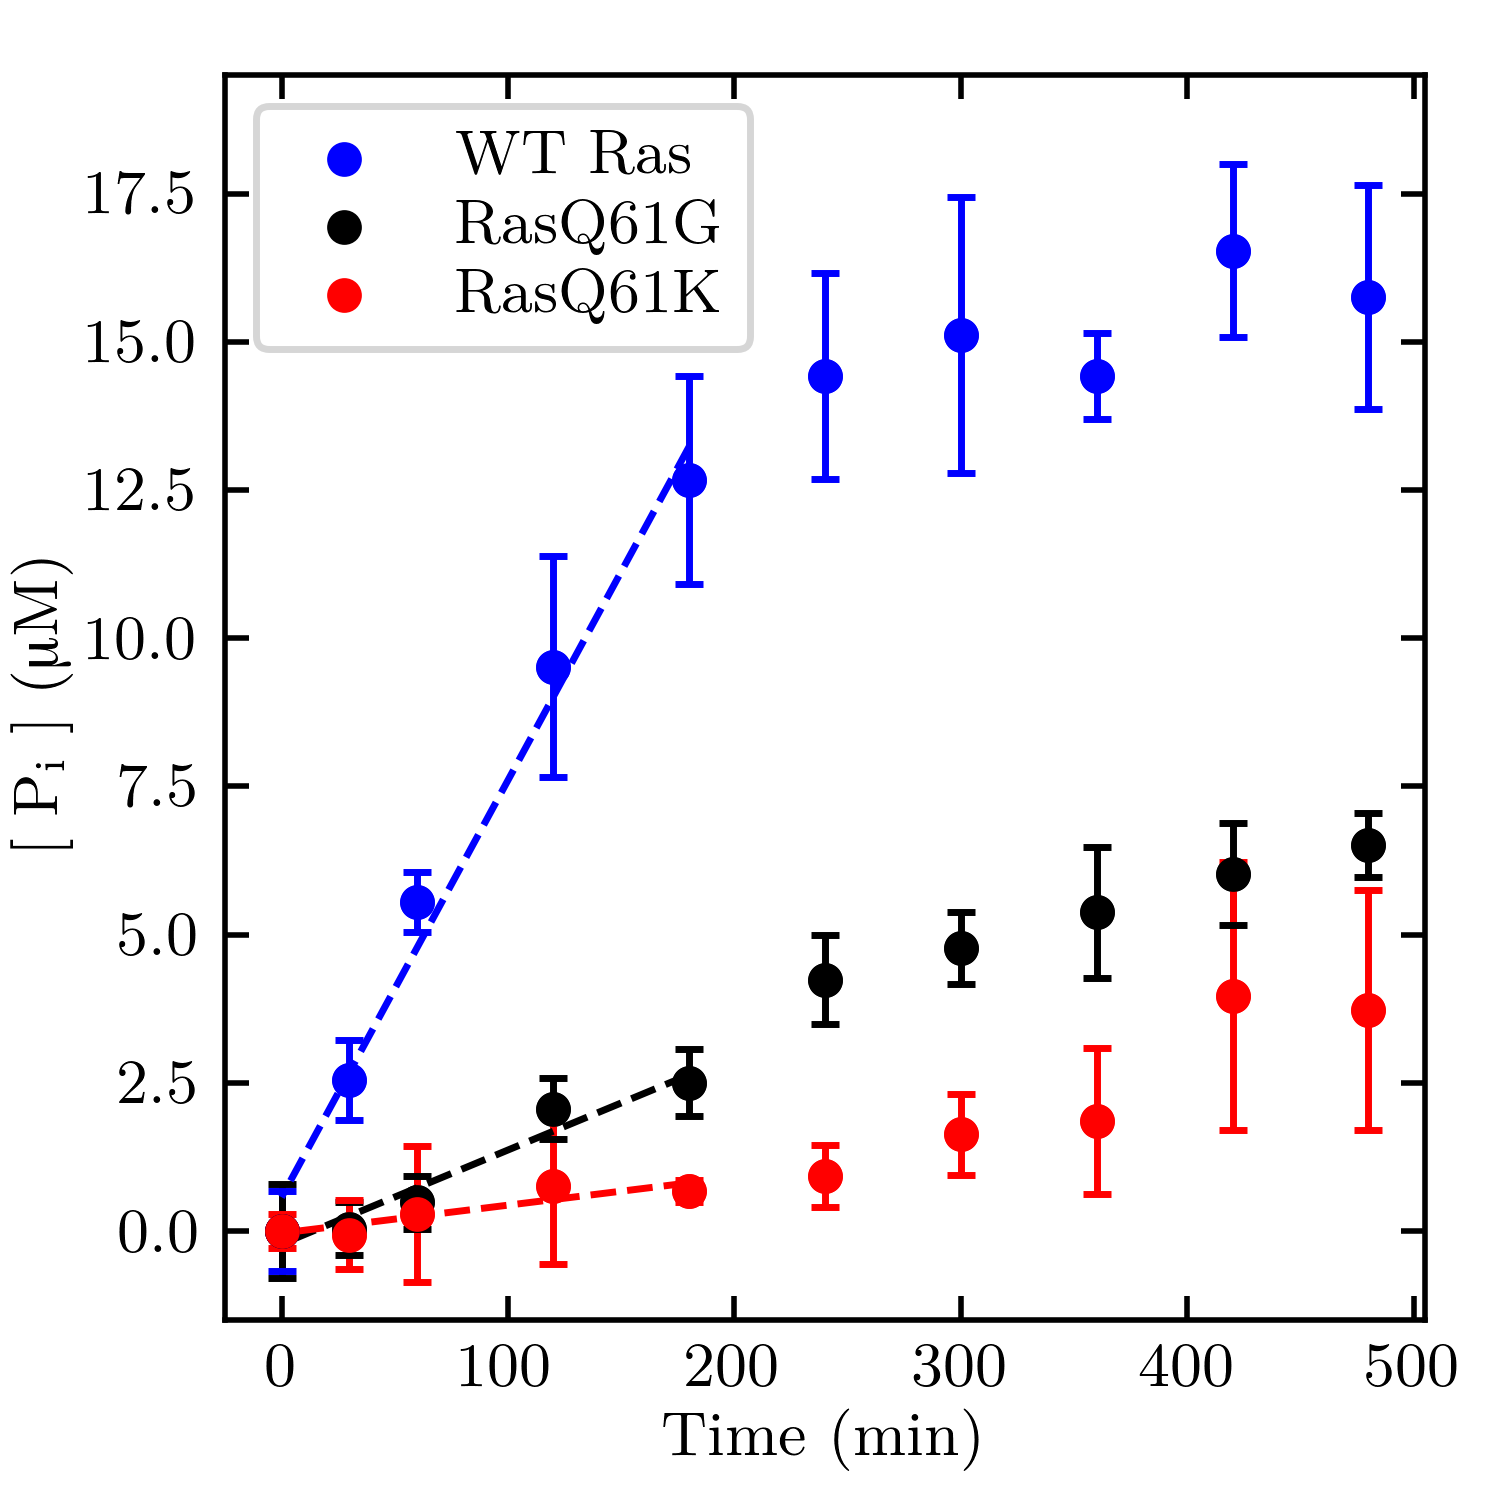
\includegraphics[width=\single]{figures-ras/modelCurvesFigure.png}
    \caption[Representative kinetic measurements of RasQ61X constructs]{
        Representative kinetic measurements of 4 $\mu$M RasQ61X constructs reacted with 20 $\mu$M GTP over 8 h, WT (blue), Q61G (black), and Q61K (red). 
        The dashed lines represent the linear fit to the first five time points. 
        The slope of the linear fit is the initial rate of the intrinsic hydrolysis reaction. 
        The rates for each mutant are reported in Table \ref{tbl:ras-data}.}
    \label{fig:ras-curves}
\end{figure}

Though the most common approach to enzyme kinetics is the Michaelis-Menten formalism \cite{Michaelis1913, Johnson2011}, in this case, the mutations at position 61 should affect the turnover rate of the enzyme ($k_{\text{cat}}$) and not the overall Michaelis constant ($K_m$). 
Because of this, measuring the initial rate at a single substrate concentration was sufficient, given the number of constructs we investigated. 
Because initial rates depend on a variety of conditions including protein and substrate concentrations, buffer conditions, and temperature, all constructs were measured under exactly the same conditions, so they could be compared appropriately. 
In general, our results corroborate previously reported qualitative results that Q61X mutants tend to have significantly lower rates of intrinsic GTP hydrolysis with one notable exception: Q61Y had a faster initial rate ($9.64 \pm 1.50 \times 10^{-2}$ $\mu$M min$^{-1}$) than the WT ($7.03 \pm 0.49 \times 10^{-2}$ $\mu$M min$^{-1}$). 
However, all other Q61X mutant rates were slower than WT. 
Q61V had a moderate hydrolysis rate of $3.51 \pm 0.38 \times 10^{-2}$ $\mu$M min$^{-1}$. 
However, this construct precipitated after 3 h, suggesting that while the initial rate was faster than other mutations, the protein was less stable. 
The other 14 mutants we measured had initial rates of intrinsic GTP hydrolysis of less than $2.00 \times 10^{-2}$ $\mu$M min$^{-1}$.

In order to understand these results, we sorted the mutants into categories based on the polarity and ionizability of the side chain at position 61, factors which are expected to be significant for the ability to interact with and stabilize any catalytically important water molecules in the active site. 
Residues with positively charged side chains (K and R) had measured initial rates between $0.40 \times 10^{-2}$ and $0.60 \times 10^{-2}$ $\mu$M min$^{-1}$, a 15-fold decrease in intrinsic rate from WT. 
Residues with negatively charged side chains (D and E) had measured initial rates between $0.40$ and $0.90 \times 10^{-2}$ $\mu$M min$^{-1}$, a 10- to 20-fold decrease. 
For the nonpolar residues (A, F, G, I, L, M, and V), we measured initial rates between $0.6 \times 10^{-2}$ and $1.6 \times 10^{-2}$ $\mu$M min$^{-1}$, with the exception of V for which we measured a rate of $3.51 \times 10^{-2}$ $\mu$M min$^{-1}$. 
Polar, uncharged residues (H, N, Q, S, T, W, and Y) varied much more significantly, the fastest of which were the WT (Q) measured at $7.03 \times 10^{-2}$ $\mu$M min$^{-1}$ and Y measured at $9.64 \times 10^{-2}$ $\mu$M min$^{-1}$.
Two of the larger polar residues (H and W) had measured rates of $0.92 \times 10^{-2}$ $\mu$M min$^{-1}$ and $1.19 \times 10^{-2}$ $\mu$M min$^{-1}$, respectively. 
The smaller polar residues (S and T) were among the slowest mutants with rates of $0.37 \times 10^{-2}$ $\mu$M min$^{-1}$ and $0.18 \times 10^{-2}$ $\mu$M min$^{-1}$, respectively. 
The remaining large polar mutant (N), which is the most chemically similar to the wild-type Q, had a rate of $1.32 \times 10^{-2}$ $\mu$M min$^{-1}$, approximately six times slower than the WT rate. 
Although the few published rate constants of intrinsic hydrolysis by RasQ61X mutants reported in the literature have been calculated using the Michaelis-Menten formalism, and therefore cannot be compared directly to our initial rate measurements, we report them here for convenience. 
John et al. reported rate constants of $2.8 \times 10^{-2}$ min$^{-1}$ for the WT Ras and $0.2 \times 10^{-2}$ min$^{-1}$ for RasQ61H \cite{John1988}. 
Krengel et al. reported an observed rate of $0.1 \times 10^{-2}$ min$^{-1}$ for RasQ61L \cite{Krengel1990}.
RasQ61E has been reported to have a 10-fold slower hydrolysis rate than the WT\cite{Der1986}; however, Frech et al. reported a 20-fold faster intrinsic hydrolysis rate for RasQ61E when controlling for the 100-fold larger $K_d$ values for the RasQ61E-GTP complex \cite{Frech1994}.

Recently, Stafford et al. used VSE spectroscopy to measure electric field changes due to the change in identity of the residue at RasQ61\cite{Stafford2012}. 
In those experiments, RasQ61X was docked to \RalBSCN{}, which contained a cyanocysteine vibrational probe. 
The FTIR absorption frequencies from the nitrile group on the probe when docked to each Ras mutant are listed in Table \ref{tbl:ras-data}. 
Though \RalB{} docks to GTP-bound Ras with a micromolar $K_d$, we did not expect it to have an effect on the Ras intrinsic hydrolysis rate. 
To confirm this, and in order to compare our rate results with the published VSE data, we measured the intrinsic hydrolysis rate of WT Ras alone versus WT Ras docked to \RalBSCN{} and observed no differences in the rate of intrinsic hydrolysis whether or not \RalBSCN{} was present (Figure \ref{fig:ras-ral}).

\begin{figure}
    \center
    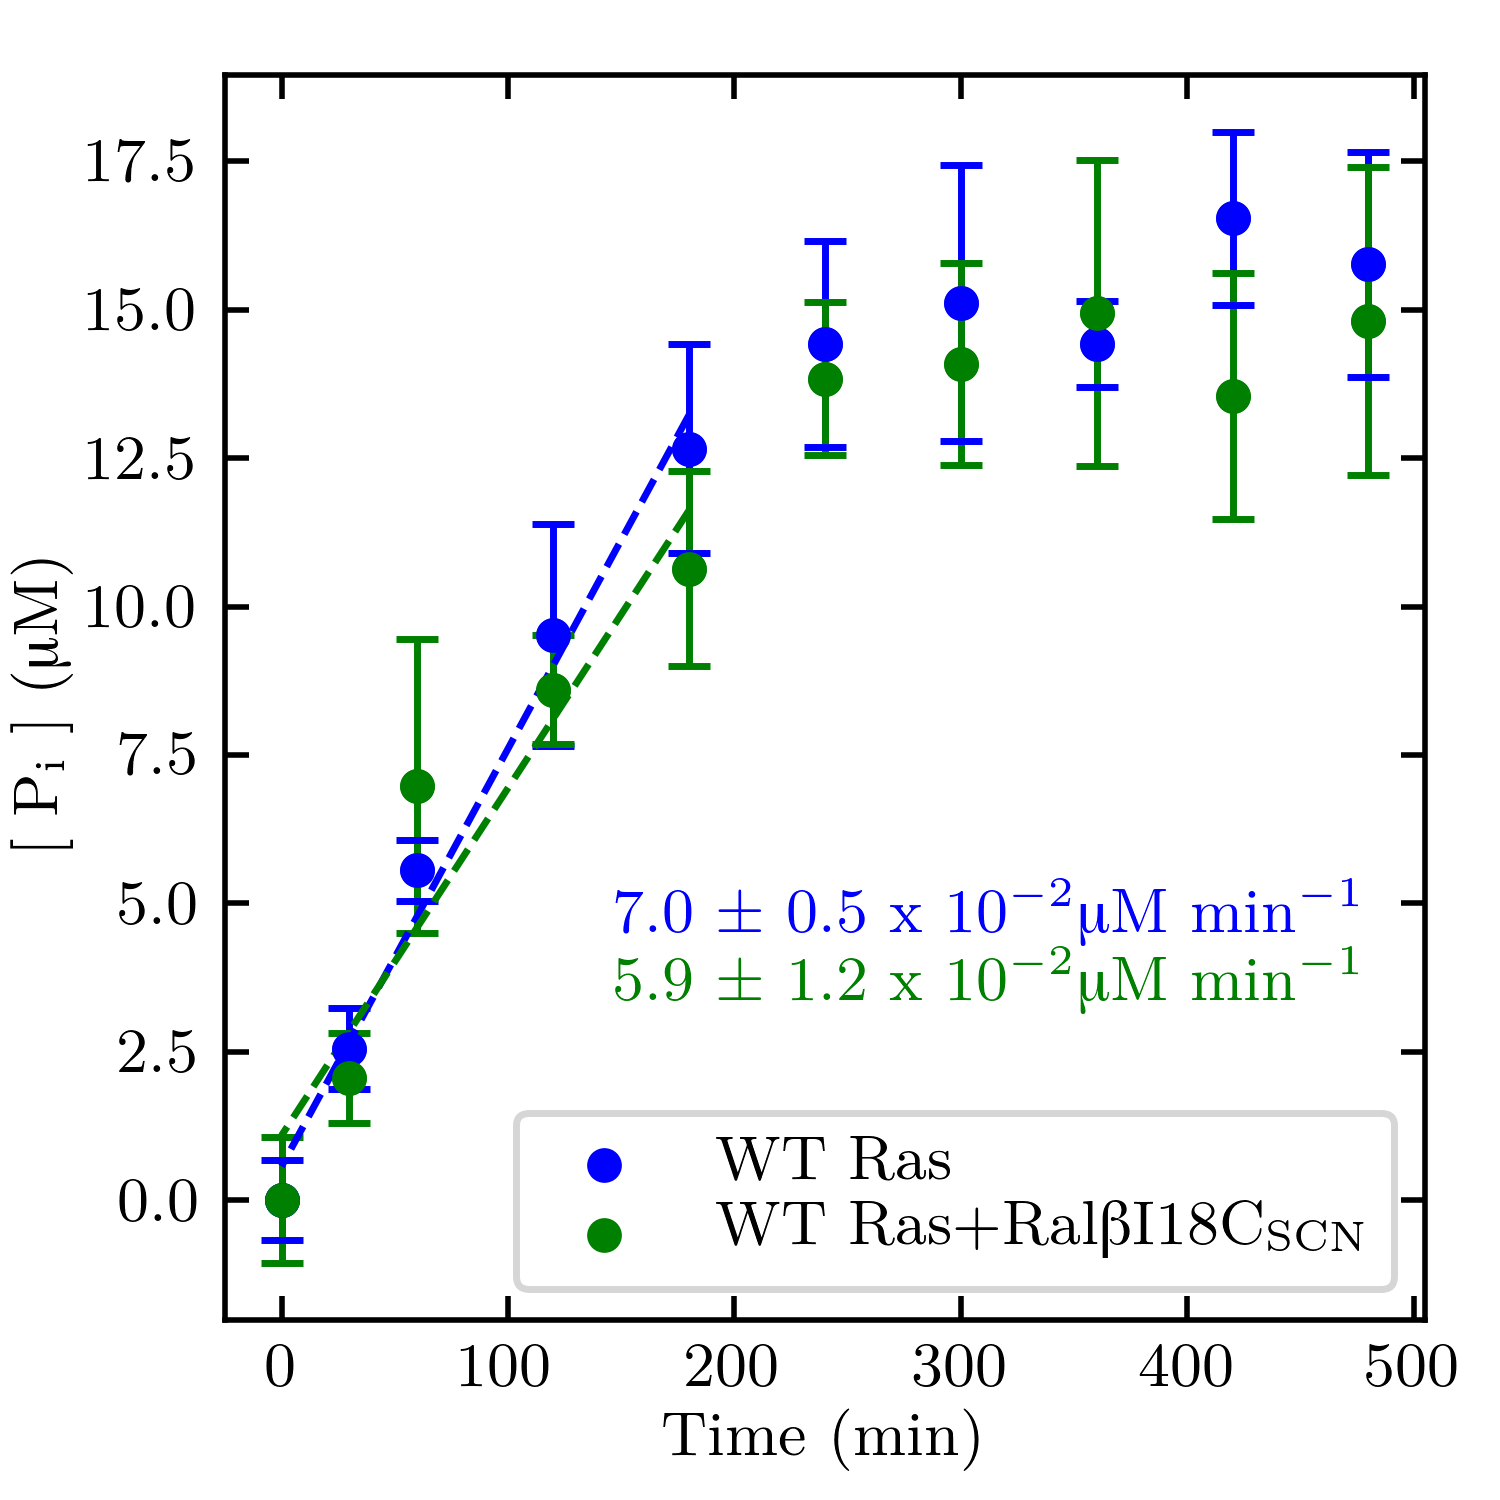
\includegraphics[width=\single]{figures-ras/Figure3.png}
    \caption[Comparison of the intrinsic Ras rate to the intrinsic Ras\RalBSCN{} rate]{
        Concentration of the phosphate product of the intrinsic hydrolysis reaction for both WT Ras (blue) and WT Ras docked to \RalBSCN{} (green) over 8 h. 
        Linear regression fits are shown to the first five time points of each data set, and the slopes are displayed in the corresponding color. 
        The intrinsic hydrolysis rate of WT Ras/\RalBSCN{} is within error of the intrinsic hydrolysis rate of WT Ras alone ($5.9 \pm 1.1 \times 10^{-2}$ $\mu$M min$^{-1}$ and $7.0 \pm 0.5 \times 10^{-2}$ $\mu$M min$^{-1}$, respectively).
    }
    \label{fig:ras-ral}
\end{figure}

\subsection{SASA calculations}

Because the proposed mechanism in Figure \ref{fig:ras-mech}A is based on a favorable interaction of Q61 with water, we attempted to quantify the likelihood of this interaction by calculating the SASA for each mutant of several subsets of atoms of the Q61X residue using the gmx sasa tool \cite{Eisenhaber1995}.
While SASA is often an oversimplification of solvent interactions, it is nevertheless a good starting point because it is efficient and convenient to calculate from a protein structure or MD trajectory. 
We therefore calculated the SASA of both the whole side chain and the polar atoms on the side chain; we refer to these quantities as the ``side chain SASA'' and the ``polar atom SASA,'' respectively. 
All N and O atoms and their bonded hydrogens were considered to be polar atoms. 
Each calculated SASA was weighted using the weighted histogram analysis method (WHAM) at 300 K, and the Boltzmann-weighted average SASA value was computed. 
These averages and standard deviations are reported in Table \ref{tbl:ras-data}.

Since F, I, L, M, and V do not have polar atoms on their side chains, the polar atom SASAs for these residues were exactly zero. 
S, T, and W all had similar polar atom SASAs of $\sim$18 \si{\angstrom^2}. 
This is not surprising, since they each have one heavy polar atom and one polar hydrogen. 
However, Y, which also has one polar heavy atom and one polar hydrogen, had a polar atom SASA of $\sim$37 \si{\angstrom^2}, more than double the other hydroxyl side chains (S and T), suggesting that the polar atoms of Y interact much more strongly with water than S or T. 
H, which has two polar heavy atoms but only one polar hydrogen, had a similar polar atom SASA of $\sim$34 \si{\angstrom^2}. 
The other two polar, uncharged residues (N and Q) have identical polar groups yet exhibited different polar atom SASAs at $\sim$49 \si{\angstrom^2} and $\sim$65 \si{\angstrom^2}. 
Similarly, the two negatively charged residues (D and E) have identical polar groups yet exhibited different polar atom SASAs at $\sim$51 \si{\angstrom^2} and $\sim$60 \si{\angstrom^2}, respectively. 
In both of these cases (N versus Q, and D versus E), the larger residue had the larger polar SASA, indicating the extra carbon in the side chain allowed the polar atoms to extend further from the backbone and interact more with solvent. 
Finally, we calculated a polar atom SASA for K that was similar to that of N and D ($\sim$50 \si{\angstrom^2}), and we calculated the largest polar atom SASA for R (which has the most polar atoms) of $\sim$71 \si{\angstrom^2}.

We also calculated the side chain SASAs for all mutants and compared them to the polar atom SASAs. 
Unsurprisingly, because of their relative size, S and T had the lowest side chain SASAs at $47 \pm 9$ \si{\angstrom^2} and $59 \pm 11$ \si{\angstrom^2},respectively. 
D, N,and V all had similar side chain SASAs at $77 \pm 7$ \si{\angstrom^2}, $76 \pm 10$ \si{\angstrom^2}, and $78 \pm 11$ \si{\angstrom^2}, respectively, despite D and T having about the same molecular volume.
This indicates that the polar side chain of T spent more time interacting with the protein than D, and less time interacting with water. 
Residues M, L, E, I, and Q all had intermediate side chain SASAs that fell between 91 \si{\angstrom^2} and 101 \si{\angstrom^2}. 
Residues F, H, K, and R had larger side chain SASAs at $114 \pm 21$ \si{\angstrom^2}, $108 \pm 14$ \si{\angstrom^2}, $114 \pm 22$ \si{\angstrom^2},and $121 \pm 24$ \si{\angstrom^2}, respectively. 
This is surprisingly low for R, indicating that the positively charged side chain interacted favorably with the surrounding protein but not available water molecules.
Finally, residues W and Y had the largest side chain SASA values at $151 \pm 21$ \si{\angstrom^2} and $130 \pm 25$ \si{angstrom^2}. 
While such a large value is unsurprising for W since the residue is so large, 130 \si{\angstrom^2} is nearly the maximum surface area for Y, indicating a very favorable interaction with the solvent environment. 
Combined, the SASA calculations indicated that residues similar in size and chemical identity can still partition differently in water based on the local chemical structure of the protein near position 61 and therefore make different contributions both to the electric field and the distribution of water in the active site. 

%%%%%%%%%%%%%%%%%%%%%%%%%%%%%%%%%%%%%%%%%%%%%%%%%%%%%%%%%%%%%%%%
%%%%%%%%%%%%%%%%%%%%%%%%%%%%%%%%%%%%%%%%%%%%%%%%%%%%%%%%%%%%%%%%
\section{Discussion}\label{ras-discussion}
%%%%%%%%%%%%%%%%%%%%%%%%%%%%%%%%%%%%%%%%%%%%%%%%%%%%%%%%%%%%%%%%
%%%%%%%%%%%%%%%%%%%%%%%%%%%%%%%%%%%%%%%%%%%%%%%%%%%%%%%%%%%%%%%%

Because the proposed mechanism of intrinsic hydrolysis of GTP in Ras (Figure \ref{fig:ras-mech}A) relies on electrostatic stabilization of a transient hydronium ion in the active site, we plotted the measured vibrational frequencies from Stafford et al.\cite{Stafford2012} against the measured initial rates of intrinsic hydrolysis (Figure \ref{fig:ras-stark_vs_rate}). 
Since hydrolysis rates change by nearly 2 orders of magnitude, it is useful to view these differences in rate on a logarithmic scale. 
For the polar and negatively charged residues, which are capable of stabilizing the proposed hydronium ion, the rates increased rapidly with increasing nitrile absorption frequency until $\sim$2163 \si{\wn}, the absorption energies of Ras containing both Q (i.e., WT) and Y at position 61, and then rapidly decreased with the continued increase in absorption frequency. 
This correlation was fit to a normal distribution with the residues capable of stabilizing the hydronium ion (the polar and negatively charged residues). 
For these data, residues that caused the nitrile absorption frequency to red-shift or blue-shift from $\sim$2163 \si{\wn} decreased the rate.

\begin{figure}
    \center
    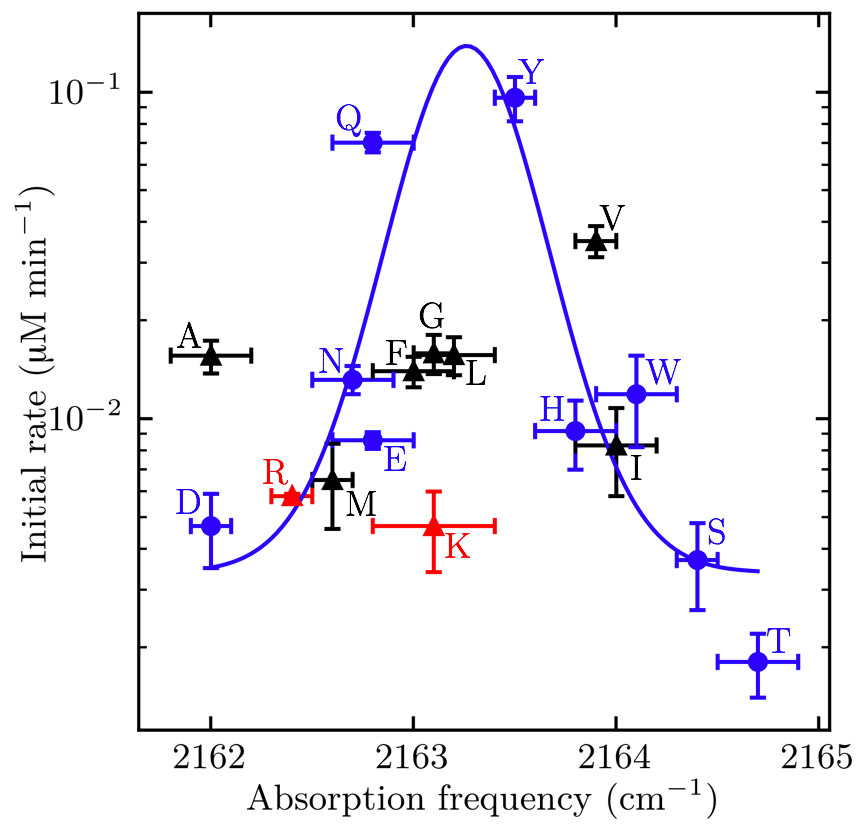
\includegraphics[width=\single]{figures-ras/Figure4.png}
    \caption[Vibrational frequencies compared to the measured intrinsic rate of hydrolysis]{
        Vibrational frequencies of the nitrile on \RalBSCN{} against the log of the measured intrinsic rate of GTP hydrolysis. 
        Blue: polar and negatively charged side chains. Black: all nonpolar side chains. 
        Red: the two positively charged side chains. Blue line: normal distribution fit to the polar and the negatively charged side chains. 
        All points that were excluded from the fit are marked with triangles.
    }
    \label{fig:ras-stark_vs_rate}
\end{figure}

Because nitrile groups have been shown to report on changes in solvation due to hydrogen bonding, we calculated the SASA of the nitrile on \RalBSCN{} and the number of waters within a 5 \si{\angstrom} sphere of the nitrile. 
These values were within error of each other for all of the Q61X mutants and are presented in Table \ref{tbl:ras-sasa}. 
Further, because the solvation effect is caused by changes in specific hydrogen bonding interactions\cite{Choi2008}, we calculated the geometries of each observed hydrogen bond between the nitrile and solvent. 
Recently, we have shown that the geometry of these interactions can dominate the vibrational frequency\cite{First2018}.
In this case, however, the average angles and distances of the hydrogen bonding interactions were all within error of each other for each of the 18 mutant systems, as shown in Table \ref{tbl:ras-sasa}. 
Together, these data demonstrate that the perturbation to the solvation environment caused by the mutation has relaxed over the $\sim$9 \si{\angstrom} distance between the nitrile probe and position 61. 
We have previously demonstrated that, in cases of a similar hydrogen bonding environment, such as these systems, shifts in nitrile frequency agree with independent measurements of electric field \cite{Slocum2016, Slocum2017}.
We therefore interpret the shifts in absorption frequency as a measure of change in the electric field through eq \ref{eq:ras-stark}.

\begin{table}
    \caption[Nitrile exposure to water in the Ras/\RalBSCN{} constructs]{
        Boltzmann-weighted averages of the SASA of the nitrile on \RalBSCN{}, 
        number of waters within a 5 \si{\angstrom} sphere of the nitrogen of the nitrile, and 
        geometric properties of all the hydrogen bonding interaction between the solvent and the nitrile in the simulations. 
        These geometric properties are illustrated in Figure \ref{fig:ras-hbond}.
    }
    \begin{center}
    \begin{tabular}{cccccc} 
    \toprule
        \rowcolor{lgray}
        Ras Construct & SASA (\si{\angstrom^2})  & \# waters & $\left < \theta_1 \right >$  & $\left < \theta_2 \right >$ & $\left < d_{\rm{NH}} \right >$ (\si{\angstrom}) \\
    
        \cmidrule(r){1-1}\cmidrule(lr){2-2}\cmidrule(lr){3-3}\cmidrule(lr){4-4}\cmidrule(lr){5-5}\cmidrule(l){6-6}
    
    RasQ61D  & $51 \pm 13$  &  $14 \pm 2$    &  $135.2 \pm 19.3$ & $152.3 \pm 13.5$  & $2.1 \pm 0.2 $              \\  
    RasQ61E  & $60 \pm 13$  &  $15 \pm 2$    &  $133.5 \pm 19.3$ & $152.2 \pm 13.6$  & $2.1 \pm 0.2 $              \\  
    RasQ61F  & $51 \pm 17$  &  $14 \pm 3$    &  $137.3 \pm 19.4$ & $153.2 \pm 13.1$  & $2.1 \pm 0.2 $              \\  
    RasQ61H  & $48 \pm 15$  &  $14 \pm 3$    &  $137.4 \pm 19.3$ & $152.9 \pm 13.4$  & $2.1 \pm 0.2 $              \\  
    RasQ61I  & $58 \pm 15$  &  $15 \pm 3$    &  $134.6 \pm 18.9$ & $152.6 \pm 13.5$  & $2.1 \pm 0.2 $              \\  
    RasQ61K  & $56 \pm 16$  &  $15 \pm 3$    &  $135.1 \pm 19.6$ & $152.9 \pm 13.2$  & $2.1 \pm 0.2 $              \\  
    RasQ61L  & $57 \pm 17$  &  $15 \pm 3$    &  $135.5 \pm 18.8$ & $153.1 \pm 13.6$  & $2.1 \pm 0.2 $              \\  
    RasQ61M  & $48 \pm 18$  &  $13 \pm 3$    &  $136.9 \pm 19.3$ & $153.3 \pm 13.0$  & $2.1 \pm 0.2 $              \\  
    RasQ61N  & $52 \pm 17$  &  $14 \pm 3$    &  $135.1 \pm 19.3$ & $152.3 \pm 13.6$  & $2.1 \pm 0.2 $              \\  
    RasQ61Q  & $55 \pm 19$  &  $14 \pm 3$    &  $137.2 \pm 19.1$ & $153.0 \pm 13.3$  & $2.1 \pm 0.2 $              \\  
    RasQ61R  & $61 \pm 19$  &  $15 \pm 3$    &  $135.3 \pm 19.1$ & $152.7 \pm 13.5$  & $2.1 \pm 0.2 $              \\  
    RasQ61S  & $53 \pm 16$  &  $13 \pm 3$    &  $132.0 \pm 18.6$ & $152.6 \pm 13.7$  & $2.1 \pm 0.2 $              \\  
    RasQ61T  & $45 \pm 19$  &  $13 \pm 3$    &  $134.8 \pm 19.6$ & $152.7 \pm 13.7$  & $2.1 \pm 0.2 $              \\  
    RasQ61V  & $53 \pm 17$  &  $15 \pm 3$    &  $136.9 \pm 19.3$ & $153.7 \pm 13.1$  & $2.1 \pm 0.2 $              \\  
    RasQ61W  & $62 \pm 15$  &  $15 \pm 3$    &  $136.3 \pm 18.9$ & $151.8 \pm 13.7$  & $2.1 \pm 0.2 $              \\  
    RasQ61Y  & $56 \pm 18$  &  $14 \pm 3$    &  $135.8 \pm 19.0$ & $152.4 \pm 13.5$  & $2.1 \pm 0.2 $              \\  
    
    \bottomrule
    \end{tabular}
    \end{center}
    \label{tbl:ras-sasa}
\end{table}

\begin{figure}
    \center
    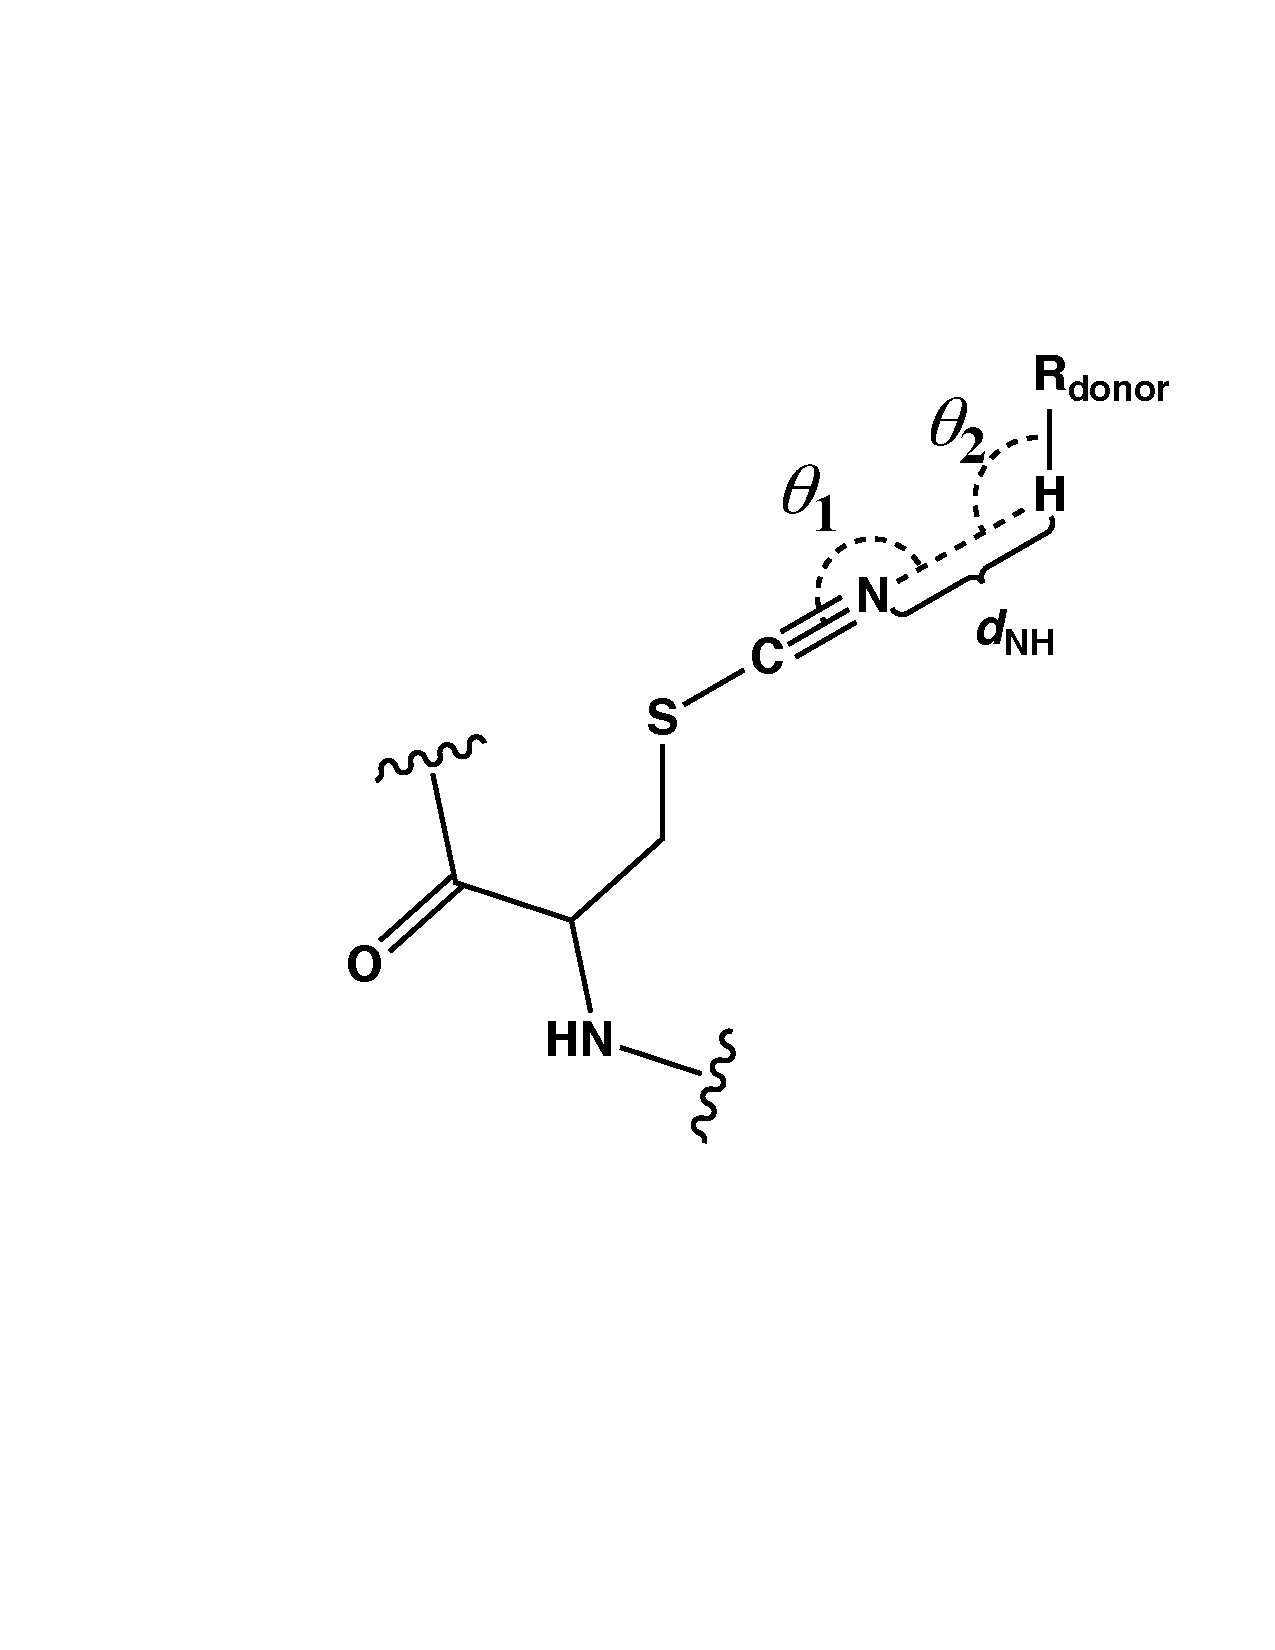
\includegraphics[width=\single]{figures-ras/Figure_S4.pdf}
    \caption[Geometric criteria for the hydrogen bonding calculations]{
        Geometric criteria and property definitions for the hydrogen bonding calculations. 
        $\theta_1$ is the C--N$\cdots$H angle, $\theta_2$ is the N$\cdots$H--R$_{\text{donor}}$ angle, where R$_{\text{donor}}$ represents a water hydrogen bond donor, and $d_{\text{NH}}$ is the distance between the hydrogen and the acceptor nitrogen. 
        To be considered a hydrogen bond, $\theta_1$ must be greater than \ang{99}, $\theta_2$ must be greater than \ang{120}, and $d_{\text{NH}}$ must be less than 2.45 \si{\angstrom}. 
        Adopted from ref \citenum{First2018}.
    } 
    \label{fig:ras-hbond}
\end{figure}

The observation in Figure \ref{fig:ras-stark_vs_rate} supports the hypothesis that the role of Q61 is to provide an electrostatic contribution to the stabilization of water near the active site and that Q61X mutants that do not provide the optimal electrostatic potential; i.e., all mutants studied besides Q and Y are less effective at stabilizing the catalytic hydronium ion. 
Mutations that caused a deviation from the optimal field in either direction (measured as a red- or blue-shift in the nitrile vibrational frequency) disrupted the intrinsic mechanism and decreased the rate, except for residues that did not stabilize a hydronium ion, resulting in rates that are normally distributed about an optimal electric field.

For the residues that would be unable to stabilize the hydronium ion in the active site, no such trend was observed. 
Two of the uncorrelated residues are R and K, the two positively charged amino acids (red data points in Figure \ref{fig:ras-stark_vs_rate}). 
These two side chains are incapable of stabilizing a hydronium ion due to Coulombic repulsion and are thus easily explained. 
The hydrophobic residues at position 61 display a more interesting behavior, however, with a range of hydrolysis activities depending on the identity of the hydrophobic residue (black data points in Figure \ref{fig:ras-stark_vs_rate}). 
For example, V has an intermediate initial rate of intrinsic hydrolysis ($3.51 \pm 0.38$ $\mu$M min$^{-1}$), while M has a very low initial rate ($0.65 \pm 0.19$ $\mu$M min$^{-1}$).  
Side chain size alone does not explain this observation: G, A, V, and L increase in molecular volume in that order, but the rates of GTP hydrolysis in those Q61X mutants do not follow the same trend.

In order to investigate the effect of side chain size, we plotted the polar atom SASA and the side chain SASA for each mutant against the nitrile shift and the initial rate of GTP hydrolysis. 
As observed in Stafford et al., the SASA of the polar atoms are well correlated with the measured vibrational frequency of the nearby nitrile on \RalBSCN{} (Figure \ref{fig:ras-sasa}A). 
With increased sampling and increased accuracy of the SASA calculation, our correlation ($r = -0.89$) is improved compared to the previous result \cite{Stafford2012}. 
Therefore, the measured field observed by the nitrile is a good measure of the ability of Q61X to interact with water and thus a good metric by which to evaluate the hypothesis of Buhrman et al. 
No correlation was observed between the polar atom SASA and the measured intrinsic rate (Figure \ref{fig:ras-sasa}B), and when we measured the side chain SASA, we found that it did not correlate to the nitrile shifts (Figure \ref{fig:ras-sasa}C). 
However, we found that the SASA of the side chain was moderately correlated (Figure \ref{fig:ras-sasa}D, $r = 0.81$) to the measured initial rate of the side chains capable of stabilizing the hydronium ion (the polar and negatively charged residues), with the exception of W. 
Because of the unique chemical structure of W, the side chain SASA was extremely large, yet the large SASA of W did not translate to a large number of water molecules in the active site of the protein. 
This prompted us to calculate how many water molecules were actually present in the GTP binding site based on the identity of the residue at position 61.

\begin{figure}
    \center
    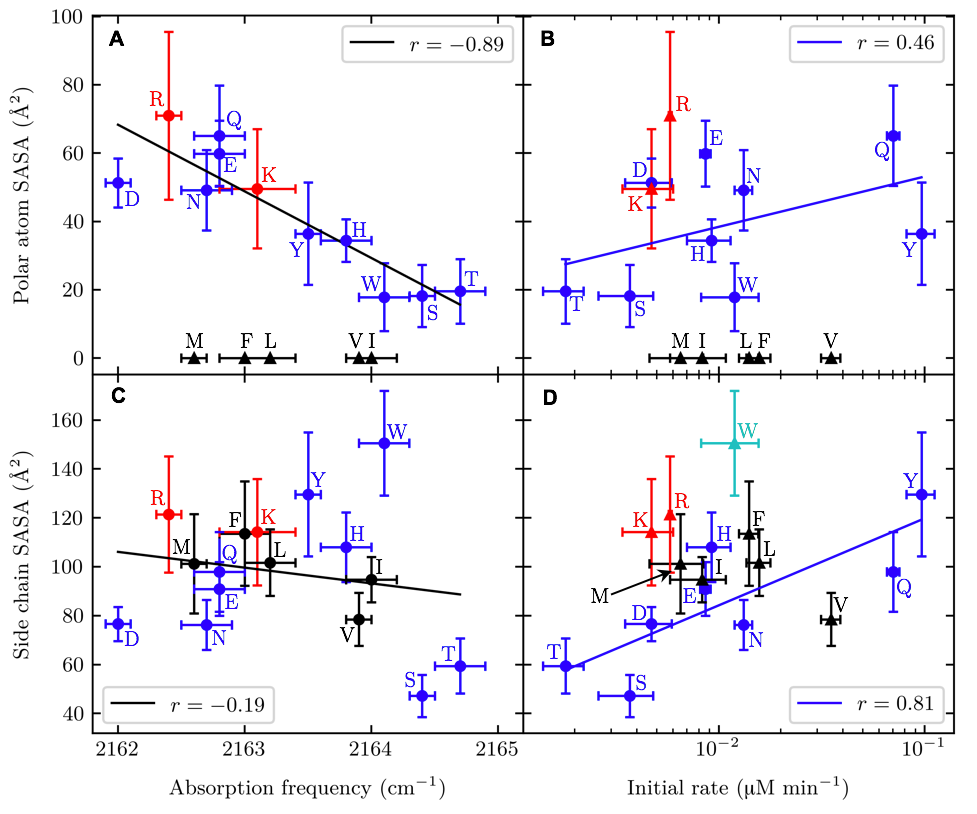
\includegraphics[width=\double]{figures-ras/Figure5.png}
    \caption[Boltzmann-weighted SASA calculations against experimentally measured frequencies and rates]{
        Boltzmann-weighted polar atom and side chain SASAs compared to experimentally measured values of nitrile absorption frequency and initial rate of intrinsic hydrolysis in RasQ61X mutants. 
        (A) The absorption frequency of the nitrile on \RalBSCN{} against the polar atom SASA of Q61X. 
        (B) The initial rate of intrinsic hydrolysis against the polar atom SASA of Q61X. 
        (C) The absorption frequency of the nitrile on \RalBSCN{} against the side chain SASA of Q61X. 
        (D) The initial rate of intrinsic hydrolysis against the side chain SASA of Q61X. 
        Blue: polar or negatively charged side chain. 
        Red: positively charged side chains. 
        Black: nonpolar side chains. 
        Triangles: residues not included in the linear regression. 
        In panel D, W (cyan) is excluded from the polar residue group as discussed in the text.
    }
    \label{fig:ras-sasa}
\end{figure}

While SASA is a convenient measure of the ability of a residue to interact with water, it lacks molecular level details of the interaction. 
Specifically, it does not address how much solvent is actually interacting with the residue. 
Instead, it only estimates the area of a residue that could interact with solvent. 
Because of this distinction and the observation that W interacted with a small number of waters, we calculated the number of waters that are confined to the active site around GTP. 
All waters that were within 5 \si{\angstrom} of GTP's reactive terminal phosphate oxygen (O1G) atom and within 5 \si{\angstrom} of the side chain of Q61 were considered to be in the active site. 
We have plotted the Boltzmann-weighted average number of water molecules that met these criteria against the log of the measured intrinsic rate in Figure \ref{fig:ras-scount}. 
We found that the number of waters in the active site was strongly correlated ($r = 0.93$) to the log of the measured intrinsic rate for residues that are capable of stabilizing the proposed hydronium ion; that is, for polar residues and negatively charged residues. 
We interpret the observation of this strong correlation to mean that the ability of the residue at position 61 to interact with water impacts the intrinsic hydrolysis rate.

\begin{figure}
    \center
    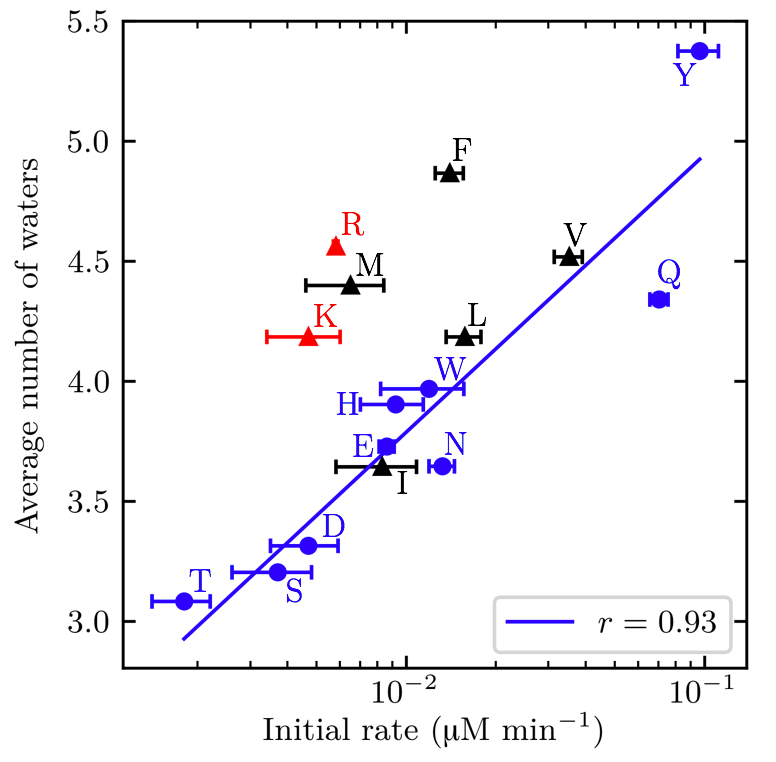
\includegraphics[width=\single]{figures-ras/Figure6.png}
    \caption[Number of waters in the active site against the measured intrinsic rate]{
        Boltzmann-weighted average number of waters in the active site per frame against the measured intrinsic rate. 
        To be considered in the active site, each water needed to be within 5 \si{\angstrom} of the Q61X side chain and within 5 \si{\angstrom} of the terminal phosphate oxygen of GTP (atom name O1G). 
        Blue: all polar or negatively charged side chains. 
        All other points are marked as triangles and are excluded from the fit. 
        Red: positively charged side chains. 
        Black: nonpolar side chains.
    }
    \label{fig:ras-scount}
\end{figure}

The positively charged residues (R and K) and the nonpolar residues (M, F, V, L, and I) are not included in the linear regression fit. 
Interestingly, it appears that the three branched nonpolar residues I, L, and V do still fit this same trend (including these residues in the fit does not change the correlation). 
However, without a concrete reason to include I, L, and V and exclude M and F, we have decided to omit all nonpolar residues from the trend. 
Indeed, if we consider the hydration potential of each residue as reported by Wolfenden et al.\cite{Wolfenden1981}, which quantifies the free energy of the transfer of the side chain from the vapor phase to buffered water, this distinction becomes even more interesting. 
When calculated in a vacuum, M and F are the only hydrophobic residues for which the transfer from the vapor phase to the solution phase occurs spontaneously, with negative hydration potentials (-1.48 and -0.76 kcal mol$^{-1}$, respectively, at pH 7), while, under the same conditions, the other hydrophobic residues I, L, and V had positive hydration potentials (2.15, 2.28, and 1.99 kcal mol$^{-1}$, respectively, at pH 7). 
This suggests that these two outliers have higher affinities for water and are changing the organization of water in the active site in some manner that is different from the other nonpolar residues. 
It is interesting that the positively charged and nonpolar residues had nonzero intrinsic hydrolysis rates, despite being unable to stabilize the transient hydronium ion. 
Without more information, it is impossible to determine if the rates are merely shifted from the correlation in Figure \ref{fig:ras-scount}, or if these mutants hydrolyzed GTP via an alternative mechanism that does not rely on the stabilization of a hydronium ion in the transition state.

Nevertheless, these results strongly support a multiwater intrinsic hydrolysis mechanism, such as the one shown in Figure \ref{fig:ras-mech}A, in which Q61 electrostatically stabilizes a hydronium ion in the transition state caused by the nucleophilic attack of a basic water molecule. 
In the case of the mechanism proposed by Buhrman et al., the hydronium ion is thought to be located between Q61, the bridging oxygen to the $\gamma$-phosphate, and a terminal oxygen on the $\gamma$-phosphate. 
This location was originally proposed based on observations from a crystal structure, which, by necessity, were obtained with the nonhydrolyzable GTP analogue 5'-guanylylimidodiphosphate (GppNHp) in the binding site. 
It is generally thought that the conversion of the bridging oxygen to a nitrogen between the second and third phosphate is a fairly conservative change, and it has allowed for the study of GTPases in the ON state. 
In the case of the VSE measurements by Stafford et al., which also relied on GppNHp, there should be very little difference in the results between GTP-bound Ras and GppNHp-bound Ras because the only observable perturbation at this distance should be electrostatic. 
However, the effect on the hydrogen bonding network caused by the switch of an oxygen to a nitrogen in the phosphate region may not be negligible. 
Indeed, in every one of our simulations of Q61X constructs with GTP, the bridging oxygen accepts a hydrogen bond from the amide backbone of G12. 
The interaction distances and number of hydrogen bonds per frame between these two groups are shown in Table \ref{tbl:ras-g12}. 
However, this interaction is not present in the crystal structure of Buhrman et al. 
The replacement of GTP with GppNHp in the crystallization replaces a hydrogen bond accepting oxygen (the bridging oxygen) with a hydrogen bond donating nitrogen, which could push G12 farther from the $\gamma$-phosphate, providing room for a water to be observed in between G12 and GppNHp. 
In our simulations, however, the hydrogen bond between G12 and GTP brings the protein backbone too close to allow for a water in this location. 
Therefore, while our data supports a multiwater mechanism in which Q61 electrostatically stabilizes a hydronium ion, which in turn stabilizes the transition state, we hypothesize that the hydronium ion must be elsewhere.

\begin{table}
    \caption[Interactions between GTP and residue G12 in Ras]{
        Interaction distances and probability of a hydrogen bond per frame between the amide nitrogen of G12 and the bridging oxygen (OS3) of GTP. 
        The standard deviations of the probabilities are omitted because they are of the same order of magnitude as the probabilities.
    }
    \begin{center}
    \begin{tabular}{ccc}
    \toprule
   \rowcolor{lgray}
    Ras construct & Interaction distance & Hydrogen bond probability\\
    \cmidrule(r){1-1}\cmidrule(rl){2-2}\cmidrule(l){3-3}
Q61D  & $2.86 \pm   0.12$ &   $0.54 $\\%\pm   0.50$  \\
Q61E  & $2.99 \pm   0.14$ &   $0.52 $\\%\pm   0.50$  \\
Q61F  & $2.87 \pm   0.12$ &   $0.50 $\\%\pm   0.50$  \\
Q61H  & $2.89 \pm   0.13$ &   $0.65 $\\%\pm   0.48$  \\
Q61I  & $2.90 \pm   0.14$ &   $0.71 $\\%\pm   0.45$  \\
Q61K  & $2.90 \pm   0.13$ &   $0.70 $\\%\pm   0.46$  \\
Q61L  & $2.88 \pm   0.13$ &   $0.47 $\\%\pm   0.50$  \\
Q61M  & $2.87 \pm   0.12$ &   $0.50 $\\%\pm   0.50$  \\
Q61N  & $2.86 \pm   0.12$ &   $0.52 $\\%\pm   0.50$  \\
Q61Q  & $2.85 \pm   0.11$ &   $0.53 $\\%\pm   0.50$  \\
Q61R  & $2.89 \pm   0.13$ &   $0.67 $\\%\pm   0.47$  \\
Q61S  & $2.88 \pm   0.12$ &   $0.49 $\\%\pm   0.50$  \\
Q61T  & $2.89 \pm   0.13$ &   $0.73 $\\%\pm   0.44$  \\
Q61V  & $2.89 \pm   0.14$ &   $0.43 $\\%\pm   0.50$  \\
Q61W  & $2.91 \pm   0.14$ &   $0.76 $\\%\pm   0.43$  \\
Q61Y  & $2.87 \pm   0.13$ &   $0.59 $\\%\pm   0.49$  \\

\bottomrule
\end{tabular}
    \end{center}
    \label{tbl:ras-g12}
\end{table}

Proposed mechanisms have also identified other residues in the region that could contribute to the intrinsic hydrolysis reaction, in particular Y32 identified in the mechanism proposed by Buhrman et al \cite{Buhrman2010}. 
Though mutant forms of residues other than G12, G13, and Q61 have not generally been identified as oncogenic, nor have they been reported as frequent mutations in tumors, Y32 is of interest to us because the Buhrman et al. mechanism suggests that it may be a secondary stabilizer of the transition state hydronium ion. 
However, our simulations were not set up to test specifically the mechanism proposed by Buhrman et al.; this is based on the crystal structure 3k8y where Y32 is oriented differently than our simulations based on 1lfd. 
Using simulations based on the crystal structure 3k8y and corresponding experiments, we are currently investigating the effect of mutations to Y32 on the intrinsic hydrolysis rate and will report these results in a later publication. 

Ultimately, the ability of each of these mutations to slow hydrolysis enough to convert Ras into an oncoprotein is based not only on its role in the intrinsic hydrolysis reaction but also on the likelihood that the DNA mutation causing these changes could occur. 
It is therefore not surprising that the oncogenic mutants of RasQ61X are also statistically the most likely to occur because they require the mutation of only a single nucleotide. 
The E, K, L, and R codons are only a single base switch away from the WT; the work described here demonstrates that any one of those changes results in a drastic suppression of intrinsic hydrolysis, leading to oncogenic effects which have been cataloged elsewhere \cite{Prior2012, Hobbs2016}. 
It has been suggested by Cox et al. that therapeutic strategies targeting the intrinsic hydrolysis mechanism of Ras may need to be mutation-specific\cite{Cox2014} and therefore require knowledge of the differences in the electrostatic contributions of these side chains. 
Our data set can be used to validate new computational models and inform future drug design efforts towards targeting the oncogenic forms of H-Ras. 

%%%%%%%%%%%%%%%%%%%%%%%%%%%%%%%%%%%%%%%%%%%%%%%%%%%%%%%%%%%%%%%%
%%%%%%%%%%%%%%%%%%%%%%%%%%%%%%%%%%%%%%%%%%%%%%%%%%%%%%%%%%%%%%%%
\section{Conclusions}\label{ras-conclusion}
%%%%%%%%%%%%%%%%%%%%%%%%%%%%%%%%%%%%%%%%%%%%%%%%%%%%%%%%%%%%%%%%
%%%%%%%%%%%%%%%%%%%%%%%%%%%%%%%%%%%%%%%%%%%%%%%%%%%%%%%%%%%%%%%%

We measured initial rates of intrinsic hydrolysis of GTP by WT Ras and 17 mutants of Q61. 
We compared the measured rates to previous measurements of nitrile probe frequency for each construct and found that polar and negatively charged residues, which are capable of stabilizing a hydronium ion, have initial rates that were normally distributed around a central nitrile frequency of $\sim$2163 \si{\wn}. 
Recently, using hybrid QM/MM simulations, Tichauer et al. arrived at a similar conclusion that also supports a multiwater mechanism for a closely related protein, N-Ras, by demonstrating that mutations at position 61 alter the distribution of waters in the active site \cite{Tichauer2018}. 
Similarly, we compared the initial rates to the average number of waters in the binding site calculated from MD simulations and showed that the number of waters in the binding site was strongly correlated with the initial rate for residues that can stabilize a hydronium ion. 
These observations support a multiwater mechanism of intrinsic hydrolysis, such as that of Buhrman et al. 
We further postulated that the proposed location of the transition state hydronium ion cannot be located at the bridging oxygen based on the observation of a hydrogen bond between G12 and GTP that was not present in the crystal structures that used the nonhydrolyzable GTP analogue, GppNHp. 
Together, these results form a data set that will be useful for validating computational models and potential future therapeutic strategies.

